\documentclass[11pt]{article}
\usepackage{fancyhdr} 
\pagestyle{fancy}
\fancyhf{}
\fancyheadoffset{0cm}
\renewcommand{\headrulewidth}{0pt} 
\renewcommand{\footrulewidth}{0pt}
\fancyhead[R]{{\color{gray!50}Page Number: \thepage}}
\fancypagestyle{plain}{%
  \fancyhf{}%
  \fancyhead[R]{\thepage}%
}




\usepackage{graphicx}
\usepackage[margin=.5in]{geometry} 
\usepackage{amsmath,amsthm,amssymb}
%\usepackage{gensymb}
  \usepackage{hyperref}
  \usepackage{pdfpages} 
  %\usepackage[table]{xcolor}
  
 %\usepackage{xcolor} % Required for specifying colors by name
\definecolor{ocre}{RGB}{52,177,201} % Define the orange color used for highlighting throughout the book

% Font Settings
\usepackage{avant} % Use the Avantgarde font for headings
%\usepackage{times} % Use the Times font for headings
\usepackage{mathptmx} % Use the Adobe Times Roman as the default text font together with math symbols from the Sym­bol, Chancery and Com­puter Modern fonts

%\usepackage{microtype} % Slightly tweak font spacing for aesthetics
%\usepackage[utf8]{inputenc} % Required for including letters with accents
\usepackage[T1]{fontenc} % Use 8-bit encoding that has 256 glyphs
%\usepackage{soul}
\usepackage{undertilde}
%\usepackage{accents}
\newcommand{\StandardLM}{\by=\bX \bbeta +{\epsilonbf}}

\usepackage{xcolor}
\usepackage{xparse}
\definecolor{lightGray}{gray}{0.95}
\definecolor{lightGrayOne}{gray}{0.9}
\definecolor{lightBlueOne}{RGB}{204, 255, 255}
\definecolor{lightBlueTwo}{RGB}{204, 238, 255}
\definecolor{lightBlueThree}{RGB}{204, 204, 255}
\definecolor{AltBlue}{RGB}{119,14,161}
\definecolor{Orchid}{RGB}{186,85,211}

\definecolor{BGBlue}{RGB}{220,221,252}
\definecolor{BGBlueOne}{RGB}{204,229,255}

\definecolor{DarkGreenOne}{RGB}{34,139,34}

\definecolor{BGGreen}{RGB}{240,243,245}
\definecolor{lightGreenOne}{RGB}{179, 255, 179}
\definecolor{lightGreenTwo}{RGB}{198, 255, 179}
\definecolor{lightGreenThree}{RGB}{243, 255, 230}
\definecolor{AltGreen}{RGB}{193, 240, 240}

\definecolor{BOGreen}{RGB}{180,0,0}
\definecolor{BGGreenOne}{RGB}{220,250,220}

\definecolor{lightBrownOne}{RGB}{255, 221, 204}
\definecolor{lightBrownTwo}{RGB}{255, 229, 204}
\definecolor{lightBrownThree}{RGB}{242, 217, 230}


\definecolor{HLTGreen}{RGB}{230,244,215}
\definecolor{ExcBrown}{RGB}{153,0,0}
\definecolor{ExcBGBrown}{RGB}{255,204,204}
\definecolor{BGYellowOne}{RGB}{255,235,208}
\definecolor{BGPink}{RGB}{255,215,240}

\newcommand{\MakeVec}[1]{{\utilde{\bf #1}}}

\NewDocumentCommand{\MCOption}{O{1.75in} m}{
\TextInBoxTwo[BGPink]{ #1 } {\TextInBoxTwo[white]{.1 in }{ \quad}\HLT{#2}}
}

 \NewDocumentCommand{\ThreeChoices}{O{Do not Know}O{Not confident}O{Confident}}{
\MCOption{#1} \MCOption{#2} \MCOption{#3}
}
 
\NewDocumentCommand{\OneBlock}{ O{HLTGreen} m m }{\colorbox{#1}{\begin{minipage}{#2} $ #3$ \end{minipage}}}

\NewDocumentCommand{\HLT}{ O{HLTGreen} m }{\colorbox{#1}{#2}}
%\NewDocumentCommand{\HLTEQ}{ O{HLTGreen} m }{\colorbox{#1}{$#2$}}
\NewDocumentCommand{\HLTEQ}{ O{white} m }{\colorbox{#1}{$#2$}}

%\newcommand{\HLT}[1]{\colorbox{HLTGreen}{#1}}
\newcommand{\DEHLT}[1]{\colorbox{lightGrayOne}{\color{white} #1}}

\newcommand{\TextInBoxOne}[2]{  {\fcolorbox{white}{lightGrayOne}{\begin{minipage}{#1}  #2 \end{minipage}}}}


\NewDocumentCommand{\TextInBoxTwo}{ O{lightGrayOne} m m } {{\fcolorbox{white}{#1}{\begin{minipage}{#2} { #3} \end{minipage}}}}


\newcommand{\TextInBox}[2]{  {\fcolorbox{BGGreen}{BGGreen}{\begin{minipage}{#1}  #2 \end{minipage}}}}
\newcommand{\TextInBoxCol}[2]{
\fcolorbox{BGBlue}{BGBlue}{%
\begin{minipage}{#1}
 {\color{AltBlue} #2}
\end{minipage}}%
}

\NewDocumentCommand{\TxtBnd}{ O{lightBrownOne} m m } {{\fcolorbox{white}{#1}{\begin{minipage}{#2} { #3} \end{minipage}}}}


\newcommand{\BandInTopBox}[2]{
\fcolorbox{AltBlue}{AltBlue}{%
\begin{minipage}{#1}{ {\color{white}  #2 \hspace{.1in}} }
\end{minipage}}%
}


\newcommand{\TextInBoxThm}[2]{
\fcolorbox{AltBlue}{lightGray}{%
\begin{minipage}{#1}
 {\color{black} #2}
\end{minipage}}%
}

\newcommand{\TextInBoxThmOne}[2]{
\fcolorbox{BGBlue}{BGBlueOne}{%
\begin{minipage}{#1}
 {\color{AltBlue} #2}
\end{minipage}}%
}

\newcommand{\TextInBoxLem}[2]{
\fcolorbox{BGBlue}{lightGray}{%
\begin{minipage}{#1}
 {\color{black} #2}
\end{minipage}}%
}



\newcommand{\TextInBoxLemOne}[2]{
\vspace{.02 in}
\noindent
\fcolorbox{BGBlue}{BGBlue}{%
\begin{minipage}{#1}
 {\color{AltBlue} #2}
\end{minipage}}%
}



\newcommand{\DefBox}[1]{
%\vspace{.1 in}
\noindent
\TextInBoxLem{4.5 in }{
\BandInTopBox{4.4 in }{}
\TextInBoxLemOne{4.4 in }{
#1
}}}





\newcommand{\DefBoxOne}[2]{
%\vspace{.1 in}
\noindent
\TextInBoxLem{4.5 in }{
\BandInTopBox{4.4 in }{#1}
\TextInBoxLemOne{4.4 in }{
#2
}}}


\newcommand{\ThmBox}[2]{
\noindent
\TextInBoxThm{4.4 in }{
\TextInBoxThmOne{4.4 in }{
#1}
#2}
}

\newcommand{\LemBox}[2]{
\noindent
\TextInBoxLem{4.5 in }{
\TextInBoxLemOne{4.4 in }{
#1}
#2}
}

\newcommand{\PropBox}[2]{
\vspace{.1 in}
\noindent
\TextInBoxLem{4.5 in }{
\TextInBoxLemOne{4.4 in }{
#1}
#2}
}




\newcommand{\TextInBoxExc}[2]{
\noindent
\fcolorbox{white}{BGGreenOne}{%
\begin{minipage}{#1}
 {\color{black} #2}
\end{minipage}}%
}


\newcommand{\TextInBoxExample}[2]{
\noindent
\fcolorbox{white}{BGPink}{%
\begin{minipage}{#1}
 {\color{black} #2}
\end{minipage}}%
}


\newcommand{\ExerciseBox}[1]{
\noindent
%\TextInBoxLem{6 in }{
\TextInBoxExc{6 in }{
#1}
%#2}
}


\newcommand{\ExampleBox}[1]{
\noindent
%\TextInBoxLem{6 in }{
\TextInBoxExample{6 in }{
#1}
%#2}
}

\NewDocumentCommand{\CommentBox}{ O{BGBlue}  m }{
\TextInBoxLem{5.5in }{
{\bf Comment:}\\
\TextInBoxLemOne{5.4 in }{
#2}}
}



\newcommand{\HLTY}[1]{\HLTEQ[yellow]{#1}}
\newcommand{\HLTW}[1]{\HLTEQ[white]{#1}}



\newcommand{\qBox}[1]{
  \begin{tikzpicture}
\node[draw=none,shade,
      top color=lightGrayOne,
      bottom color=lightGray,
      rounded corners=2pt,
      blur shadow={shadow blur steps=5}
    ] at (0,0) {    \noindent 
\fcolorbox{white}{BGBlue}{%
\begin{minipage}{4.55 in}
 {\color{black} {
 #1}}
\end{minipage}  }%
 };
 
    \end{tikzpicture}
}
 
 


 

\newcommand{\qBoxCol}[2]{
  \begin{tikzpicture}
\node[draw=none,shade,
      top color=lightGrayOne,
      bottom color=lightGray,
      rounded corners=2pt,
      blur shadow={shadow blur steps=5}
    ] at (0,0) {    \noindent
\fcolorbox{white}{#1}{%
%\begin{minipage}{4.55 in}
\begin{minipage}{4.55 in}
 {
 \color{black} {
 #2}}
\end{minipage}  }%
 };
 
    \end{tikzpicture}
}
  
  
  
  
  
  

\NewDocumentCommand{\qBrd}{O{4.55 in} m m}{
  \begin{tikzpicture}
\node[draw=none,shade,
      top color=#2,
      bottom color=#2,
      rounded corners=2pt,
      blur shadow={shadow blur steps=5}
    ] at (0,0) {    \begin{minipage}{#1}
 {
 \color{black} {
 #3}}
\end{minipage} 

 };
 
    \end{tikzpicture}
}
    
  
  
  
  
\NewDocumentCommand{\qbx}{O{4.55 in} m m}{
  \begin{tikzpicture}
\node[draw=none,shade,
      top color=lightGrayOne,
      bottom color=lightGray,
      rounded corners=2pt,
      blur shadow={shadow blur steps=5}
    ] at (0,0) {    \noindent
\fcolorbox{white}{#2}{%
%\begin{minipage}{4.55 in}
\begin{minipage}{#1}
 {
 \color{black} {
 #3}}
\end{minipage}  }%
 };
 
    \end{tikzpicture}
}
  
 
 
 \newcommand{\CurlyBox}[1]{
\begin{center}
  \begin{tikzpicture}
    \node[tape,draw=none,shade,
      top color=blue!40,
      bottom color=blue!5,
      rounded corners=1pt,
      blur shadow={shadow blur steps=5,shadow blur extra rounding=1.3pt}
    ] at (2,0){\sffamily\bfseries\large #1};
  \end{tikzpicture}
\end{center} 
 }


\newcommand{\CmntBnd}{\BandInTopBox{4.5in}{Comment:}}
\NewDocumentCommand{\TopBand}{O{Comment:} m}{ \BandInTopBox{4.5in}{#2}}

\newcommand{\DBX}[1]{
 	\HLTEQ[AltBlue]{
 				\HLTEQ[BGBlue]{  #1  }
 	}
 }



\NewDocumentCommand{\TransitionFrame}{O{slateblue}m}{
\begin{frame}{ }
\qBoxCol{#1!40}{\vspace{.8in}  \begin{center}\qBrd[2in]{#1!70}{ \begin{center} \vspace{.1in}
  #2 \\
 \vspace{.1in}
\end{center}}\end{center}
\vspace{.7in}
}

\end{frame}

}
%\newcommand{\proof}{ {\bf Proof:  } }
%\usepackage{enumerate}
%
\NewDocumentCommand{\InnerProduct}{ O{\cdot,\cdot} }{ \left\langle #1  \right\rangle  }

%\newcommand{\InnerProduct}[2]{  \left\langle #1, #2  \right\rangle }
\newcommand{\Ind}[1]{\mathbb{I}\left(#1 \right)}
\newcommand{\StandardLM}{\by=\bX \bbeta +{\epsilonbf}}
\newcommand{\StandardLMmod}{\bY=\bX \bbeta +{\epsilonbf}}
\usepackage{undertilde}
\newcommand{\MakeVec}[1]{{\utilde{\bf #1}}}
\newcommand{\Zplus}{{\Z_{+}}}
\newcommand{\Proj}[1]{{#1}\left( {#1}^T{#1}\right)^{-}{#1}^T }
\NewDocumentCommand{\YiDotDef}{O{B} m}{ \left(Y_{{#2}1},\ldots,Y_{{#2}{#1}} \right)}
\NewDocumentCommand{\YiDot}{O{i}}{  \utilde{Y}_{{#1 \bullet}}  }

\NewDocumentCommand{\OneWay}{ O{T} O{B} m}{
 \IfEqCase{#3}{%
  {model}{   Y_{ij}=\mu+ \tau_i+ \epsilon_{ij} \text{ for } i 		=1, 2,\ldots #1; j = 1,2,\ldots #2  
  	 }
  {Y}{
  \left[ {\begin{array}{c;{2pt/2pt}c;{2pt/2pt}c;{2pt/2pt}c ;{2pt/2pt}c}
   \overbrace{ Y_{11},\ldots ,Y_{1{#2}}}^{\text{Treatment 1}}  & \cdots &  \overbrace{ Y_{i1},\ldots Y_{i{#2}}}^{\text{Treatment 2}} & \cdots & \overbrace{Y_{{#1}1} \ldots Y_{{{#1}}{#2}}}^{\text{Treatment #1}} \end{array} } \right]^T 
  	 }
  	 {YInDot}{\left[ {\begin{array}{c;{2pt/2pt}c;{2pt/2pt}c;{2pt/2pt}c ;{2pt/2pt}c}
  \utilde{Y}_{1 \bullet}^T  & \cdots &   \utilde{Y}_{i \bullet}^T& \cdots & \utilde{Y}_{{#1} \bullet}^T \end{array} } \right]^T_{{#1}{#2}\times 1}
  	 }
  	 {response}{
  \left[ {\begin{array}{c;{2pt/2pt}c;{2pt/2pt}c;{2pt/2pt}c ;{2pt/2pt}c}
   \overbrace{ Y_{11},\ldots ,Y_{1{#2}}}^{\text{Treatment 1}}  & \cdots &  \overbrace{ Y_{i1},\ldots Y_{i{#2}}}^{\text{Treatment 2}} & \cdots & \overbrace{Y_{{#1}1} \ldots Y_{{{#1}}{#2}}}^{\text{Treatment #1}} \end{array} } \right]^T  
  	 }
  	 {treatments}{ \tau_1,\ldots , \tau_{#1} }
  	  {tau}{ \tau_1,\ldots , \tau_{#1} }
  	 {beta}{\left(\mu, \HLT{$\tau_1,\ldots , \tau_{#1} $}\right)^T}
  	 {error}{
  \left[ {\begin{array}{c;{2pt/2pt}c;{2pt/2pt}c;{2pt/2pt}c ;{2pt/2pt}c}
   \overbrace{ \epsilon_{11},\ldots ,\epsilon_{1{#2}}}^{\text{Treatment 1}}  & \cdots &  \overbrace{ \epsilon_{i1},\ldots \epsilon_{i{#2}}}^{\text{Treatment 2}} & \cdots & \overbrace{\epsilon_{{#1}1} \ldots \epsilon_{{{#1}}{#2}}}^{\text{Treatment #1}} \end{array} } \right]^T   
  	 }
  	 {design}{
 \left[ {\begin{array}{c;{2pt/2pt}cccc}
   \Onebf_{#2} &  \Onebf_{#2} & \ZeroF  & \ldots &  \ZeroF\\
   \Onebf_{#2} &  \ZeroF   &\Onebf_{#2} & \ldots  & \ZeroF\\
   \vdots   & \vdots    & \vdots  & \ddots & \vdots  \\
    \Onebf_{#2} & \ZeroF & \cdots  & \ldots    & \Onebf_{#2}\\
    \end{array}
   } \right] _{{#1}{#2}\times ({#1}+1)}
  }
  {designKP}{ \left[  {\begin{array}{c;{2pt/2pt}c}
   \underbrace{\Onebf_{#1}\otimes  \Onebf_{#2}} &  \underbrace{I_{#1} \otimes \Onebf_{#2} }
   \end{array} }\right]
   }
    {X}{
 \left[ {\begin{array}{c;{2pt/2pt}cccc}
   \Onebf_{#2} &  \Onebf_{#2} & \ZeroF  & \ldots &  \ZeroF\\
   \Onebf_{#2} &  \ZeroF   &\Onebf_{#2} & \ldots  & \ZeroF\\
   \vdots   & \vdots    & \vdots  & \ddots & \vdots  \\
    \Onebf_{#2} & \ZeroF & \cdots  & \ldots    & \Onebf_{#2}\\
    \end{array}
   } \right] _{{#1}{#2}\times ({#1}+1)}
  }
  {XKP}{ \left[  {\begin{array}{c;{2pt/2pt}c}
   \underbrace{\Onebf_{#1}\otimes  \Onebf_{#2}} &  \underbrace{I_{{#1}} \otimes \Onebf_{#2} }
   \end{array} }\right]
   }
   {XMu}{ \Onebf_{#1}\otimes  \Onebf_{#2} }
   {XTau}{I_{{#1}} \otimes \Onebf_{#2}}
   {ProjMat}{
   \left[ {\begin{array}{c;{2pt/2pt}c;{2pt/2pt}c ;{2pt/2pt}c}
    \HLT{$\ProjOne{#2}$}&  \ZeroF& \cdots &\ZeroF\\
   \ZeroF&  \HLT{$\ProjOne{#2}$} & \cdots & \ZeroF\\
   \vdots &\vdots  &  \vdots   & \vdots  \\
    \ZeroF&  \ZeroF & \cdots & \HLT{$\ProjOne{#2}$}
    \end{array}
   } \right]_{{#1}{#2}\times {#1}{#2} }
   }
    {ProjMatKP}{
    I_{#1}\otimes {\ProjOne{#2}}
    }
    {YColVec}{
    \left[ {\begin{array}{c}
  \utilde{Y}_{1 \bullet}\\
  \hdashline[2pt/2pt]\\
   \vdots\\
  \hdashline[2pt/2pt]\\
  \utilde{Y}_{i \bullet}\\
  \hdashline[2pt/2pt]\\
   \vdots\\
  \hdashline[2pt/2pt]\\
   \utilde{Y}_{{#1} \bullet}\\
    \end{array}
   } \right]_{{#1}{#2}\times 1}}
   {YDotBar}{\left[
   {\begin{array}{c}
  \overline{Y}_{1 \bullet}\\
  \hdashline[2pt/2pt]\\
   \vdots\\
  \hdashline[2pt/2pt]\\
  \overline{Y}_{i \bullet}\\
  \hdashline[2pt/2pt]\\
   \vdots\\
  \hdashline[2pt/2pt]\\
   \overline{Y}_{{#1} \bullet}\\
    \end{array}
   }\right]_{{#1}\times 1} }
    }  	 
}







%
%
%%\usepackage{accents}
%\newcommand{\SpaceU}{\mathcal{U}}
%\newcommand{\Span}[1]{\mathcal{L}(#1)}
%%\hypersetup{colorlinks=true}
%\newcommand{\N}{\mathbb{N}}
%\newcommand{\Z}{\mathbb{Z}}
% \newcommand{\SpaceW}{\mathcal{W}}
%\newcommand{\SpaceV}{\mathcal{V}}
%\newcommand{\real}[1]{{\mathbb R}^{#1}}
%\newcommand{\Pdg}{P_{\alphabfs (\Deltabfs_{y})}}
%\newcommand{\spn}{\mathrm{span}}
%\newcommand{\diag}{\mathrm{diag}}
\newcommand{\E}{\mathrm{E}}
\newcommand{\var}{\mathrm{Var}}
\newcommand{\cov}{\mathrm{Cov}}
\newcommand{\covhat}{\widehat{\mathrm{Cov}}}
\newcommand{\rank}{\mathrm{rank}}
\newcommand{\stack}{\mathrm{stack}}
\newcommand{\Normal}{\mathrm{Normal}}
\newcommand{\tr}{\mathrm{\,tr}}
\newcommand{\avar}{\mathrm{\,avar}}
\newcommand{\vecc}{\mathrm{\,vec}}
\newcommand{\true}{\mathrm{true}}

% Bold Face symbols
\newcommand{\vbf}{{\mathbf v}}
\newcommand{\w}{{\utilde{\mathbf w}}}
\newcommand{\X}{\mathbf X}
\newcommand{\Xhat}{\widehat{\X}}
\newcommand{\x}{{\utilde{\mathbf x}}}
\newcommand{\Y}{{\mathbf Y}}
\newcommand{\y}{\mathbf y}
\newcommand{\Xbar}{\bar{\X}}
\newcommand{\Ybar}{\bar{\Y}}
\newcommand{\ellhat}{\hat{\ell}}
\newcommand{\ellbf}{\mathbf{\ell}}
\newcommand{\ellbfhat}{\hat{\ellbf}}
\newcommand{\abf}{{\utilde{\mathbf a}}}
\newcommand{\q}{{\mathbf q}}
\newcommand{\f}{{\mathbf f}}
\newcommand{\Obf}{\mathbf O}


\newcommand{\Xcaln}{{\mathcal X}_{n}}
\newcommand{\Xbarcal}{\bar{{\mathcal X}}}
\newcommand{\Xbb}{\mathbb{X}}
\newcommand{\Fbb}{\mathbb{F}}
\newcommand{\Ybb}{\mathbb{Y}}

\newcommand{\Xbbhat}{\widehat{\mathbb{X}}}
\newcommand{\Ss}{\mathbf{S}}
\newcommand{\Ty}{\T_{y}}
\makeatletter
\renewcommand*{\@seccntformat}[1]{%
   \csname the#1\endcsname.\quad}
\makeatother
%\newcommand{\Z}{{\mathbf Z}}
\newcommand{\z}{{\mathbf z}}
\newcommand{\Zbar}{\bar{\Z}}
\newcommand{\Zhat}{\hat{\Z}}
\newcommand{\Zwidehat}{\widehat{\Z}}
\newcommand{\Sigmabfhatz}{\greekbold{\hat{\Sigma}}_{\Z}}
\newcommand{\Sigmabfhatzy}{\greekbold{\hat{\Sigma}}_{\Z|y}}
\newcommand{\Sigmabfzy}{\Sigmabf_{\Z|y}}
\newcommand{\sigmahat}{\hat{\sigma}}

\newcommand{\fit}{\mathrm{fit}}
\newcommand{\res}{\mathrm{res}}
\newcommand{\rres}{{ 11},\mathrm{res}}

\newcommand{\ffit}{{ 11},\mathrm{fit}}
\newcommand{\G}{\mathbf{G}}
\newcommand{\Ll}{\mathbf{L}}
\newcommand{\Guno}{\mathbf{G_1}}
\newcommand{\Hh}{\mathbf{H}}
\newcommand{\Ww}{\mathbf{W}}
\newcommand{\Mm}{\mathbf{M}}
\newcommand{\bw}{{\utilde{\mathbf{w}}}}


%\newcommand{\pfcpc}{PFC(PC)}
\newcommand{\pfcpc}{$\mathrm{PFC}_{\mathrm{PC}}$}
\newcommand{\pfcall}{$\mathrm{PFC}_{\mathrm{all}}$}

\newcommand{\fbf}{{\mathbf f}}
\newcommand{\fbfhat}{\hat{\fbf}}
\newcommand{\fhat}{\hat{f}}
\newcommand{\D}{\mathbf D}
\newcommand{\cbf}{{\mathbf c}}
\newcommand{\Dfbf}{\D_{\fbf}}
\newcommand{\Dfbfhat}{\D_{\fbfhat}}
\newcommand{\K}{\mathbf K}
\newcommand{\Khat}{\widehat \K}

\newcommand{\ghat}{\hat{g}}
\newcommand{\Bhat}{\widehat{\B}}
\newcommand{\Rhat}{\widehat{R}}
\newcommand{\vhat}{\widehat{\bv}}

\newcommand{\uhat}{\widehat{\bu}}
\newcommand{\gbf}{{\mathbf g}}
\newcommand{\gbfhat}{\hat{\gbf}}

\newcommand{\Dgbf}{\D_{\gbf}}
\newcommand{\Dgbfhat}{\D_{\gbfhat}}

\newcommand{\obf}{\mathbf o}
\newcommand{\Pbf}{{\mathbf P}}
\newcommand{\Qbf}{{\mathbf Q}}
\newcommand{\Qfbf}{\Qbf_{\fbf}}
\newcommand{\Qfbfhat}{\Qbf_{\fbfhat}}
\newcommand{\Qgbf}{\Qbf_{\gbf}}
\newcommand{\Qgbfhat}{\Qbf_{\gbfhat}}
\newcommand{\Pgbf}{\Pbf_{\gbf}}

\newcommand{\T}{\mathbf T}
\newcommand{\tT}{\widetilde{\T}}
\newcommand{\tV}{\widetilde{\V}}
\newcommand{\dT}{\dot{\T}}
\newcommand{\dV}{\dot{\V}}
\newcommand{\ddT}{\ddot{\T}}
\newcommand{\V}{{\mathbf V}}
\newcommand{\Vhat}{\widehat \V}
%\newcommand{\bv}{{\utilde{\mathbf v}}}
\newcommand{\bu}{{\utilde{\mathbf u}}}
\newcommand{\Vhalf}{{\mathbf V}^{\half}}
\newcommand{\tL}{{\widetilde L}}
%\newcommand{\bd}{\deltabf}

\newcommand{\ahat}{{\hat{a}}}
\newcommand{\bhat}{{\hat{b}}}

\newcommand{\U}{{\mathbf U}}
\newcommand{\tD}{{\tilde{D}}}
\newcommand{\W}{{\mathbf W}}
\newcommand{\dbf}{{\mathbf d}}
\newcommand{\Lbf}{{\mathbf L}}
\newcommand{\F}{{\mathbf F}}
\newcommand{\M}{{\mathbf M}}
%\newcommand{\N}{{\mathbf N}}
\newcommand{\s}{{\mathbf S}}
\newcommand{\sy}{{\mathbf S}_{y}}
\newcommand{\bbf}{{\utilde{\mathbf b}}}
\newcommand{\A}{{\mathbf A}}
\newcommand{\B}{{\mathbf B}}
\newcommand{\Q}{{\mathbf Q}}
\newcommand{\C}{{\mathbf C}}
\newcommand{\Chat}{\widehat{\mathbf C}}
\newcommand{\Dhat}{\widehat{\mathbf D}}
\newcommand{\e}{\utilde{\mathbf e}}
\newcommand{\Ebf}{{\mathbf E}}
\newcommand{\g}{\mathbf g}
\newcommand{\R}{{\mathbb{ R}}}
\newcommand{\Ghat}{\widehat{\G}}
\newcommand{\Hbf}{{\mathbf H}}
\newcommand{\h}{\mathbf h}
\newcommand{\tB}{\widetilde{\B}}
\newcommand{\tC}{\widetilde{\C}}
\newcommand{\mpc}{M_{\mathrm{\scriptscriptstyle{PC}}}}
\newcommand{\mpfc}{M_{\mathrm{\scriptscriptstyle{PFC}}}}
\newcommand{\lpc}{L_{\mathrm{\scriptscriptstyle{PC}}}}
\newcommand{\lpfc}{L_{\mathrm{\scriptscriptstyle{PFC}}}}
\newcommand{\tlpfc}{\widetilde{L}_{\mathrm{\scriptscriptstyle{PFC}}}}



% Greek Bold Face symbols

\newcommand{\greekbold}[1]{\mbox{\boldmath $#1$}}
\newcommand{\alphabf}{{\utilde{\greekbold{\alpha}}}}
\newcommand{\alphabfhat}{\widehat{\alphabf}}
\newcommand{\alphahat}{\widehat{\alpha}}
\newcommand{\alphabfs}{\greekbold{\scriptstyle \alpha}}
\newcommand{\etabf}{\utilde{\greekbold{\eta}}}
\newcommand{\etabftd}{\widetilde{\etabf}}
\newcommand{\etabfs}{\greekbold{\scriptstyle \eta}}
\newcommand{\betabf}{\utilde{\greekbold{\beta}}}
%\newcommand{\taubf}{\utilde{\greekbold{\tau}}}
\newcommand{\lambdabf}{\utilde{\greekbold{\lambda}}}
\newcommand{\etabfhat}{\hat{\greekbold{\eta}}}
\newcommand{\rhobf}{\greekbold{\rho}}
\newcommand{\betabfhat}{\widehat{\greekbold{\beta}}}
\newcommand{\betabfs}{\greekbold{\scriptstyle \beta}}
\newcommand{\taubfhat}{\hat{\greekbold{\tau}}}
\newcommand{\taubfn}{\taubf_{n}}
\newcommand{\taubfhatn}{\hat{\taubf}_{n}}
\newcommand{\Lambdabf}{\greekbold{\Lambda}}
\newcommand{\Lambdabfhat}{\widehat{\greekbold{\Lambda}}}
\newcommand{\Lambdabfs}{\greekbold{\scriptstyle{\Lambda}}}
\newcommand{\epsilonbf}{{\utilde{\greekbold{\epsilon}}}}
\newcommand{\mubfbar}{\bar{\mubf}}
\newcommand{\mubfhat}{\hat{\mubf}}
\newcommand{\mubfs}{{\greekbold{\scriptstyle \mu}}}
\newcommand{\J}{\mathbf J}
\newcommand{\gammabf}{\greekbold{\gamma}}
\newcommand{\gammabfhat}{\hat{\greekbold{\gamma}}}
\newcommand{\gammabfy}{\greekbold{\gamma}_{y}}
\newcommand{\Gammabf}{\greekbold{\Gamma}}
\newcommand{\Gammabft}{\widetilde{\greekbold{\Gamma}}}
\newcommand{\gammabfs}{\greekbold{{\scriptstyle \gamma}}}
\newcommand{\Gammabfs}{{\greekbold{\scriptstyle \Gamma}}}
\newcommand{\Gammabfhat}{\widehat{\greekbold{\Gamma}}}
\newcommand{\deltabf}{\greekbold{\delta}}
\newcommand{\Deltabf}{\greekbold{\Delta}}
\newcommand{\Deltabfhat}{\widehat{\greekbold{\Delta}}}
\newcommand{\Deltabfs}{{\greekbold{\scriptstyle \Delta}}}
\newcommand{\deltabfs}{{\greekbold{\scriptstyle \delta}}}
\newcommand{\Deltabfshat}{{\widehat{\greekbold{\scriptstyle \Delta}}}}
\newcommand{\omegabf}{\greekbold{\omega}}
\newcommand{\Omegabf}{\greekbold{\Omega}}
\newcommand{\Omegabft}{\widetilde{\greekbold{\Omega}}}
\newcommand{\Omegabfs}{{\greekbold{\scriptstyle \Omega}}}
\newcommand{\Omegabfstd}{{\tilde{\greekbold{\scriptstyle \Omegabf}}}}
\newcommand{\Omegabfsbar}{{\bar{\greekbold{\scriptstyle{\Omegabf}}}}}
\newcommand{\Omegabftd}{\widetilde{\Omegabf}}
\newcommand{\Omegabfbar}{\bar{\Omegabf}}
\newcommand{\Omegabfhat}{\widehat{\greekbold{\Omega}}}
\newcommand{\phibf}{\greekbold{\phi}}
\newcommand{\phibfhat}{\hat{\greekbold{\phi}}}


\newcommand{\Sigmabf}{\greekbold{\Sigma}}
\newcommand{\Sigmabfhat}{\greekbold{\widehat{\Sigma}}}
\newcommand{\Sigmabft}{\greekbold{\widetilde{\Sigma}}}
\newcommand{\Sigmabfhats}{{\greekbold{\scriptstyle \widehat{\Sigma}}}}
\newcommand{\Sigmabfs}{{\greekbold{\scriptstyle \Sigma}}}
\newcommand{\mubf}{\utilde{\greekbold{\mu}}}

\newcommand{\xibf}{\greekbold{\xi}}
\newcommand{\xibfy}{\xibf_{y}}
\newcommand{\xibfs}{{\greekbold{\scriptstyle \xi}}}
\newcommand{\xibfhat}{{\hat{\xibf}}}
\newcommand{\xibfhats}{\hat{\xibfs}}

\newcommand{\xibfhaty}{{\hat{\xibf}_{y}}}
\newcommand{\txibf}{\tilde{\greekbold{\xi}}}
\newcommand{\txibfs}{\tilde{\greekbold{\scriptstyle \xi}}}
\newcommand{\Phibf}{\greekbold{\Phi}}
\newcommand{\Phibfhat}{\widehat{\Phibf}}
\newcommand{\Phibfs}{\greekbold{\scriptstyle \Phi}}
\newcommand{\Phibfshat}{\hat{\Phibfs}}
%\newcommand{\thetabf}{\utilde{\greekbold{\theta}}}
\newcommand{\varepsilonbf}{\greekbold{\varepsilon}}

\newcommand{\zetabf}{\greekbold{\zeta}}
\newcommand{\tzetabf}{\tilde{\greekbold{\zeta}}}
\newcommand{\zetabfhat}{{\hat{\zetabf}}}
\newcommand{\zetabfs}{{\greekbold{\scriptstyle \zeta}}}
\newcommand{\zetabfhats}{\hat{\zetabfs}}
\newcommand{\nubf}{\greekbold{\nu}}
\newcommand{\nubfhat}{{\hat{\nubf}}}

\newcommand{\lambdahat}{\hat{\lambda}}
\newcommand{\ic}{(i)}

\newcommand{\fa}[1]{2{#1}}
\newcommand{\fb}[1]{1{#1}}
\newcommand{\Si}[1]{\Gammabf_{#1}\Omegabf_{#1}\Gammabf_{#1}^{T}}
\newcommand{\Sinv}[1]{\Gammabf_{#1}\Omegabf_{#1}^{-1}\Gammabf_{#1}^{T}}


%subspace notation
\newcommand{\syx}{\mathcal{S}_{Y|\X}}
\newcommand{\syz}{\mathcal{S}_{Y|\Z}}
\newcommand{\spc}{{\mathcal S}}
\newcommand{\spchat}{\widehat{\mathcal S}}
\newcommand{\dist}{{\mathcal D}}
\newcommand{\Mhat}{\widehat{{\mathbf M}}}
\newcommand{\Mhatsir}{\widehat{\mathbf M}_{\mathrm{\scriptscriptstyle{SIR}}}}
\newcommand{\Msir}{\mathbf{M}_{\mathrm{\scriptscriptstyle{SIR}}}}
\newcommand{\Msave}{\mathbf{M}_{\mathrm{\scriptscriptstyle{SAVE}}}}
\newcommand{\Mhatsave}{\widehat{\mathbf M}_{\mathrm{\scriptscriptstyle{SAVE}}}}
\newcommand{\ospc}{{\mathcal O}}
\newcommand{\hspc}{{\mathcal H}}
\newcommand{\gspc}{{\mathcal G}}
\newcommand{\mspc}{{\mathcal M}}
\newcommand{\ols}{\mathrm{ols}}
\newcommand{\pfc}{\mathrm{pfc}}
\newcommand{\mse}{\mathrm{MSE}}
\newcommand{\bspc}{\mathcal B}
\newcommand{\espc}{{\cal E}}
\newcommand{\vspc}{{\mathcal V}}
\newcommand{\iseb}{{\cal IE}_{\Sigmabfs}(\bspc)}
\newcommand{\seb}{{\cal E}_{\Sigmabfs}(\bspc)}
\newcommand{\sebhat}{\widehat{{\cal E}}_{\Sigmabfs}(\bspc)}
\newcommand{\sebp}{{\cal E}_{\Sigmabfs}(\bspc_{1})}
\newcommand{\indep}{\;\, \rule[0em]{.03em}{.67em} \hspace{-.25em}
\rule[0em]{.65em}{.03em} \hspace{-.25em}
\rule[0em]{.03em}{.67em}\;\,}
\newcommand{\iespc}{{\cal IE}}
\newcommand{\isebp}{{\cal IE}_{\Sigmabfs}^{\perp}(\bspc)}
\newcommand{\isebjhat}[1]{\widehat{{\cal IE}}_{\Sigmabfs}(\bspc)}
%\newcommand{\ZeroF}{{\bf 0}}
\newcommand{\Onebf}{{\utilde{\bf 1}}}
%\newcommand{\Onebf}{ {\underaccent{\sim}{\bf 1}}}
%\newcommand{\Ll}{\underaccent{\sim}{ l}}
%\newcommand{\ZeroF}{ {\underaccent{\sim}{\bf 0}}}
\newcommand{\ZeroF}{{\utilde{\bf 0}}}
\newcommand{\ProjOne}[1]{\frac{\Onebf_{#1} \Onebf_{#1}^T}{#1} }
\newcommand{\ProjOneK}{\frac{\Onebf_K \Onebf_K^T}{K} }

%\newtheorem{prop}{Proposition}
%\newtheorem{lemma}{Lemma}
%\newtheorem{Lemma}{Lemma}
%\newtheorem{proof}{Proof}



\newcommand{\bI}{ { \bf I }}
%\newcommand{\bX}{ \utilde{ \bf X }}
%\newcommand{\bx}{ {\utilde{ \bf x }}}
%\newcommand{\bY}{ \utilde{ \bf Y }}
%\newcommand{\bt}{ \utilde{ \bf t }}
%\newcommand{\by}{ {\utilde{ \bf y} }}
%\newcommand{\bZ}{ \utilde{ \bf Z }}
%\newcommand{\bz}{ {\utilde{ \bf z }}}
\newcommand{\bzero}{ {\utilde{ \bf 0 }}}
\newcommand{\ba}{ \utilde{ \textit{\textbf{a}}}}
\newcommand{\bb}{ \utilde{ \textit{\textbf{b}}}}
\newcommand{\EE}{\text{E}}
\newcommand{\Var}{\text{Var}}
\newcommand{\bbeta}{\utilde{\boldsymbol \beta}}
\newcommand{\bOmega}{\mbox{\boldmath{$\Omega$}}}
\newcommand{\bpsi}{\mbox{\boldmath{$\psi$}}}
\newcommand{\btheta}{\utilde{\boldsymbol \theta}}
\newcommand{\sC}{ {\cal C} }
\newcommand{\sM}{ {\cal M} }
\newcommand{\sX}{ {\cal X} }
\newcommand{\sY}{ {\cal Y} }
\newcommand{\sZ}{ {\cal Z} }
\newcommand{\ee}[1]{\mathrm{e}^{ #1 }}
\newcommand{\pr}{\text{pr}}
\newcommand{\RE}{\mathbb{R}}
\newcommand{\bigqm}[1][1]{\text{\larger[#1]{\textbf{?}}}}

\newcommand{\vsa}{\vspace{.05 in}}
\newcommand{\vsb}{\vspace{2 em}}
\newcommand{\vsc}{\vspace{1 em}}
\usepackage{color,soul}


\newcommand*\bigcdot{\mathpalette\bigcdot@{.7}}
%\newcommand*\bigcdot@[2]{\mathbin{\vcenter{\hbox{\scalebox{#2}{$\m@th#1\bullet$}}}}}
\makeatother
 
 \newcommand{\RowVecSymbol}[2]{  \left(\begin{array}{c}\rvert\\{#1}_{#2,\bigcdot}\\\rvert\end{array}\right)  }
 \newcommand{\ColumnVecSymbol}[2]{  \left(\begin{array}{c}\rvert\\{#1}_{\bigcdot,#2}\\\rvert\end{array}\right)  }
 \newcommand{\ColumnVecSymbolNoBracket}[2]{  \begin{array}{c}\rvert\\{#1}_{\bigcdot,#2}\\\rvert\end{array} }
  \newcommand{\ColumnVecAll}[3]{  \left(\begin{array}{c} {#1}_{1,#2}\\\vdots\\{#1}_{#3,#2}\end{array}\right)  }
  \newcommand{\ColumnVecAllNoBracket}[3]{  \begin{array}{c} {#1}_{1,#2}\\\vdots\\{#1}_{#3,#2}\end{array}  }
  \newcommand{\RowVecAll}[3]{  \left(\begin{array}{c} {#1}_{#2,1}\\\vdots\\{#1}_{#2,#3}\end{array}\right)  }
  \newcommand{\Vector}[2]{  \left(\begin{array}{c}{#1_{}}\\{}\\{} \end{array}\right)  }
% 
% 
%\newenvironment{definition}[2][Definition]{\begin{trivlist}
%\item[\hskip \labelsep {\bfseries #1}\hskip \labelsep {\bfseries #2.}]}{\end{trivlist}}
%

%\newenvironment{theorem}[2][Theorem]{\begin{trivlist}
%\item[\hskip \labelsep {\bfseries #1}\hskip \labelsep {\bfseries #2.}]}{\end{trivlist}}
%\newenvironment{lemma}[2][Lemma]{\begin{trivlist}
%\item[\hskip \labelsep {\bfseries #1}\hskip \labelsep {\bfseries #2.}]}{\end{trivlist}}
%\newenvironment{exercise}[2][Exercise]{\begin{trivlist}
%\item[\hskip \labelsep {\bfseries #1}\hskip \labelsep {\bfseries #2.}]}{\end{trivlist}}

\newenvironment{reflection}[2][Reflection]{\begin{trivlist}
\item[\hskip \labelsep {\bfseries #1}\hskip \labelsep {\bfseries #2.}]}{\end{trivlist}}
%\newenvironment{proposition}[2][Proposition]{\begin{trivlist}
%\item[\hskip \labelsep {\bfseries #1}\hskip \labelsep {\bfseries #2.}]}{\end{trivlist}}
%
%\newenvironment{corollary}[2][Corollary]{\begin{trivlist}
%\item[\hskip \labelsep {\bfseries #1}\hskip \labelsep {\bfseries #2.}]}{\end{trivlist}}
%\newcommand{\TextInBox}[2]{\fbox{\begin{minipage}{#1} #2 \end{minipage}}}
  \newcommand{\MatrSpace}[2]{\R^{{#1}\times {#2}}}

\newcommand{\IfAndOnlyIfArrow}{\stackrel{\text{  if and only if}}{\Longleftrightarrow}}

\newcommand{\IffArrow}{\IfAndOnlyIfArrow}



\newcommand \rbind[1]{%
    \saveexpandmode\expandarg
    \StrSubstitute{\noexpand#1}{,}{&}[\fooo]%
    %\StrSubstitute{\fooo}{,}{&}[\fooo]%
    \StrSubstitute{\fooo}{;}{\noexpand\\}[\fooo]%
    \StrSubstitute{\fooo}{:}{\noexpand\\}[\fooo]%
    \restoreexpandmode
   \left[ \begin{matrix}\fooo\end{matrix}\right]
    }
    
    
    
   \newcommand \ColVec[1]{%
    \saveexpandmode\expandarg
    \StrSubstitute{\noexpand#1}{,}{\noexpand\\}[\fooo]%
    %\StrSubstitute{\fooo}{,}{&}[\fooo]%
    \StrSubstitute{\fooo}{;}{\noexpand\\}[\fooo]%
    \StrSubstitute{\fooo}{:}{\noexpand\\}[\fooo]%
    \restoreexpandmode
   \left[ \begin{matrix}\fooo\end{matrix}\right]
    }
     \newcommand \RowVec[1]{%
    \saveexpandmode\expandarg
    \StrSubstitute{\noexpand#1}{,}{&}[\fooo]%
    %\StrSubstitute{\fooo}{,}{&}[\fooo]%
    \StrSubstitute{\fooo}{;}{&}[\fooo]%
    \StrSubstitute{\fooo}{:}{&}[\fooo]%
    \restoreexpandmode
   \left[ \begin{matrix}\fooo\end{matrix}\right]
    }



  \newcommand \Row[1]{%
    \saveexpandmode\expandarg
    \StrSubstitute{\noexpand#1}{,}{&}[\fooo]%
    %\StrSubstitute{\fooo}{,}{&}[\fooo]%
    \StrSubstitute{\fooo}{;}{&}[\fooo]%
    \StrSubstitute{\fooo}{:}{&}[\fooo]%
    \restoreexpandmode
    \begin{matrix}\fooo\end{matrix}
    }
        
    
    
    
    \newcommand \Col[1]{%
    \saveexpandmode\expandarg
    \StrSubstitute{\noexpand#1}{,}{\noexpand\\}[\fooo]%
    %\StrSubstitute{\fooo}{,}{&}[\fooo]%
    \StrSubstitute{\fooo}{;}{\noexpand\\}[\fooo]%
    \StrSubstitute{\fooo}{:}{\noexpand\\}[\fooo]%
    \restoreexpandmode
    \begin{matrix}\fooo\end{matrix}
    }

%%%%%%%%%%%%%%%%%%%%% Experimental %%%%%%%%%%%%%%%%%


\ExplSyntaxOn
\DeclareExpandableDocumentCommand{\replicate}{O{}mm}
 {
  \int_compare:nT { #2 > 0 }
   {
    {#3}\prg_replicate:nn {#2 - 1} { #1#3 }
   }
 }
\ExplSyntaxOff


\ExplSyntaxOn
\DeclareExpandableDocumentCommand{\repdiag}{O{}mm}
 {
  \int_compare:nT { #2 > 0 }
   {
    {\prg_replicate:nn {#2}{#3#1}}{#3}
   }
 }
\ExplSyntaxOff


\newcommand \StrRowDiag[1]{%
    \saveexpandmode\expandarg
    \StrSubstitute{\noexpand#1}{,}{&}[\fooo]%
    %\StrSubstitute{\fooo}{,}{&}[\fooo]%
    \StrSubstitute{\fooo}{;}{&}[\fooo]%
    \StrSubstitute{\fooo}{:}{&}[\fooo]%
    \StrCount{\fooo}{&}[\countfooo]
    \restoreexpandmode
    \repdiag[0]{\countfooo+1}{{,}}
   %\left[ \begin{matrix}\fooo\end{matrix}\right]
    }


\newcommand \DiagStrOne[2]{%
    \saveexpandmode\expandarg
    \StrSubstitute{\noexpand#1}{,}{\noexpand#2}[\fooo]%
    \restoreexpandmode
   %\left[ \begin{matrix}\fooo\end{matrix}\right]
   \fooo
    }
    
    \newcommand \DiagStr[1]{%
    \DiagStrOne{#1}{{\StrRowDiag{#1}}}
    }


%$\rbind{\replicate[,]{10}{\Col{\replicate[;]{7}{0}}}}$

%$\Col{1,2,3}$
%$\ColVec{\replicate[;]{5}{B}}$
%$ \StrRowDiag{1,2} $

%$\DiagStr{1,2,3}$

%\repdiag[-]{3}{A}
\ExplSyntaxOn
\NewDocumentCommand{\Split}{ m m o }
 {
  \tarass_split:nn { #1 } { #2 }
  \IfNoValueTF { #3 } { \tl_use:N } { \tl_set_eq:NN #3 } \l_tarass_string_tl
 }

\tl_new:N \l_tarass_string_tl

\cs_new_protected:Npn \tarass_split:nn #1 #2
 {
  \tl_set:Nn \l_tarass_string_tl { #2 }
  % we need to start from the end, so we reverse the string
  \tl_reverse:N \l_tarass_string_tl
  % add a comma after any group of #1 tokens
  \regex_replace_all:nnN { (.{#1}) } { \1\, } \l_tarass_string_tl
  % if the length of the string is a multiple of #1 a trailing comma is added
  % so we remove it
  \regex_replace_once:nnN { \,\Z } { } \l_tarass_string_tl
  % reverse back
  \tl_reverse:N \l_tarass_string_tl
 }
\ExplSyntaxOff

%%%%%%%%%%%%%%%%%%%%%%%%%%%%%%%%

\newcommand{\ShowRowMatrix}[3]{ \left[ {\begin{array}{ccc}
  \line(1,0){22} &{#1} &  \line(1,0){22} \\
     & \vdots& \\
  \line(1,0){22}  &{#2}& \line(1,0){22} \\
   &  \vdots & \\
    \line(1,0){22} &{#3}& \line(1,0){22}  \\
    \end{array}
   } \right]}
 


\newcommand{\ShowColMatrix}[3]{ \left[ {\begin{array}{ccccc}
  \line(0,1){25} & &\line(0,1){25} &  &  \line(0,1){25} \\
  {#1}  & \ldots & {#2} &\ldots   &{#3} \\
 \line(0,1){25} &  & \line(0,1){25}  &  &  \line(0,1){25} \\
    \end{array}
   } \right]}
   
   
   
   
\newcommand{\ShowRowVector}[1]{ \left[ {\begin{array}{ccc}
  \line(1,0){25} &{#1} &  \line(1,0){25} 
    \end{array}
   } \right]}   
   
   
\newcommand{\ShowColVector}[1]{ \left[ {\begin{array}{c}
  \line(0,1){25} \\    {#1} \\   \line(0,1){25}     \end{array}  } \right]}
  
\newcommand{\ColVector}[3]{ \left[ {\begin{array}{c}
  {#1}\\ \vdots \\    {#2}\\ \vdots\\{#3}  \end{array}  } \right]}
  
  
  
  
  
\newcommand{\EqSetThree}[3]{ \left\{ {\begin{array}{c}
  {#1}\\ \vdots \\    {#2}\\ \vdots\\{#3}  \end{array}  } \right.}  
  



\newcommand{\MatrixTypeA}[3]{ \left[ {\begin{array}{ccc}
 {#1}_{1,1} & \cdots & {#1}_{1,{#3}}   \\
  {#1}_{2,1} & \cdots & {#1}_{2,{#3}}   \\
    \vdots  & \ddots& \vdots  \\
     {#1}_{{#2},1} & \cdots & {#1}_{{#2},{#3}}   \\
    \end{array}
   } \right]}
 
\newcommand{\MatrixTypeAKronecker}[4]{ \left[ {\begin{array}{ccc}
 {#1}_{11}{#4} & \cdots & {#1}_{1{#3}}{#4}   \\
  {#1}_{21} {#4} & \cdots & {#1}_{2{#3}} {#4}   \\
    \vdots  & \ddots& \vdots  \\
     {#1}_{{#2}1} {#4} & \cdots & {#1}_{{#2}{#3}} {#4}   \\
    \end{array}
   } \right]}
 



\newcommand{\ShowIMat}{ {\begin{array}{cccc}
 1&  &  &    \\
  & 1 &  &  \\
    &  & \ddots &    \\
     & & & 1   \\
    \end{array}
   } }
 
\newcommand{\ShowVecOne}{
\begin{array}{c}
 1\\ 1 \\    1  
\end{array}
}

 
\newcommand{\ShowUnitVecOne}{
\begin{array}{c}
 1\\ 0 \\   0  
\end{array}
}


\newcommand{\ShowUnitVecTwo}{
\begin{array}{c}
 0\\ 1 \\   0  
\end{array}
}


\newcommand{\ShowUnitVecThree}{
\begin{array}{c}
 0\\ 0\\   1  
\end{array}
}

\newcommand{\ShowZeroThree}{
\begin{array}{c}
 0\\ 0\\   0 
\end{array}
}


\newcommand{\TwoBlockMatrix}[2]{\left[  {\begin{array}{c;{2pt/2pt}c}
   {#1} &  {#2}
   \end{array} }\right]}
   
   \newcommand{\TwoBlockMatrixH}[2]{\left[  {\begin{array}{c}
   {#1} \\
   \hdashline[2pt/2pt]
    {#2}
   \end{array} }\right]}
   
   \newcommand{\TwoBlockH}[2]{ {\begin{array}{c}
   {#1} \\
   \hdashline[2pt/2pt]
    {#2}
   \end{array} }}
   
   
\newcommand{\TwoBlock}[2]{ {\begin{array}{c;{2pt/2pt}c}
   {#1} &  {#2}
   \end{array} }}
   

      
   
   
   
 \newcommand{\ThreeBlockColVec}[3]{
   \left[ {\begin{array}{c}
  #1\\
  \hdashline[2pt/2pt]\\
   \vdots\\
  \hdashline[2pt/2pt]\\
  #2\\
  \hdashline[2pt/2pt]\\
   \vdots\\
  \hdashline[2pt/2pt]\\
   #3\\
    \end{array}
   } \right]
   }



\NewDocumentCommand{\ColDyn}{>{\SplitList{;}}m}
   {
     \left[\begin{array}{c}
       \ProcessList{#1}{ \inserColtitem }
     \end{array}\right]
   }
   \newcommand \inserColtitem[1]{ #1 \\}


\makeatletter
\newcommand{\ColDynAlt}[2][r]{%
  \gdef\@VORNE{1}
  \left[\hskip-\arraycolsep%
    \begin{array}{#1}\vekSp@lten{#2}\end{array}%
  \hskip-\arraycolsep\right]}

\def\vekSp@lten#1{\xvekSp@lten#1;vekL@stLine;}
\def\vekL@stLine{vekL@stLine}
\def\xvekSp@lten#1;{\def\temp{#1}%
  \ifx\temp\vekL@stLine
  \else
    \ifnum\@VORNE=1\gdef\@VORNE{0}
    \else\@arraycr\fi%
    #1%
    \expandafter\xvekSp@lten
  \fi}
\makeatother


\NewDocumentCommand{\eVec}{m O{}}{\MakeVec{e}_{#1, (#2)}}

\NewDocumentCommand{\Ones}{O{3}}{\Col{\replicate[,]{#1}{1}}}
\NewDocumentCommand{\Zeros}{O{3}}{\Col{\replicate[,]{#1}{0}}}
\input{../MacroDefs/Altstructure} 
 
\usepackage{tfrupee}
 \begin{document}
 \title{United Arab Emirates University \vspace{-.2in}}%replace X with the appropriate number
\author{\Large   STAT 101\\\Large  Final Exam 
} %if necessary, replace with your course title
\date{ \vspace{-.15in}$ \text{30}^{\text{th}} $ November, 2023}

%\date{ \vspace{-.2in} \small   ${23}^{\text{rd}}$ October,  2023}
 \maketitle\vspace{-.41in}
  \noindent
  %%%%%%%%%%%%%%%%%
   \thispagestyle{empty}%%%%%%%%%%%%%%%%%
%%%%%%%%%%%%%%%%% 
 \TextInBoxTwo[lightBlueThree]{6.9 in }{\Large \bf Name:\HLT[white]{ \huge \color{white}A \hspace{5.12in}\vspace{2 in}}}\\
  \TextInBoxTwo[lightBlueThree]{6.9 in }{\Large \bf  Student ID:\HLT[white]{ \huge \color{white}A \hspace{4.5in}\vspace{2 in}}}\\
% \noindent
% \TextInBox{6 in }{Name: \vspace{.1 in}}\\
% \vspace{.1in}
 

\TextInBoxTwo[lightBlueThree]{6.5in}{
\begin{itemize}
\vspace{.1in}
\item \TextInBoxTwo[white]{5.8in}{\large There  are a total of 110 points in this Question Paper. Answer as much as you can.   If your acquired score is greater than equal to 100  it will be counted as $100\%$.}\\\hspace{.2in}\\
\item \TextInBoxTwo[white]{5.8in}{\large There are three parts in this Exam.  Part-I involves TRUE/FALSE or Multiple Answer type questions,   Part-II contains a few short answer type questions }\\\hspace{.2in}\\
\item \TextInBoxTwo[white]{5.8in}{\large The Exam is scheduled for 120 minutes }\\\hspace{.2in}\\
%\item   \TextInBoxTwo[white]{5.8in}{\large There are three $\star$ marked problems that are more involved than the rest.  In case you are stuck in one of those,  you may consider solving other problems first and then continue with the $\star$ marked problems.}\\\hspace{.2in}\\
\item   \TextInBoxTwo[white]{5.8in}{\large You may take help from the  "Exam Assistance Note" containing a few required definitions and formula.   }\\\hspace{.2in}\\
\end{itemize}
}
\vspace{-.01in}

\TextInBoxTwo[lightBlueTwo]{6.5in}{ \centering For instructor's use only \vspace{.01in}\\
 \;\hspace{.4in} 
\TextInBoxTwo[white]{5.5in}{
{\Large 
\begin{center}
\begin{tabular}{| c| c| c| }
\hline
 Problem Number  & Obtained Score & Total Score \\ 
 \hline \hline
 Problem 1 &  & 40 \\  
 \hline
 Problem 2 &  & 20 \\  
 \hline
  Problem 3 &  &  10\\  
 \hline
   Problem 4 &  & 20  \\  
 \hline
    Problem 5 &  &  20\\  
 \hline
%    Problem 6 &  &  \\  
% \hline
%    Problem 7 &  &  \\  
%   \hline
%    Problem 8 &  &  \\     
 \hline
  \hline
    TOTAL &  &110  \\   
    \hline
  \hline
   TOTAL(out of 100) & \vspace{.2in} &100  \\   
 \hline \hline
\end{tabular}
\end{center}
}}\vspace{.12in}
}





\newpage
\vspace{1in}{\begin{center} \color{gray!30}You May Use This Page for Rough Work\end{center}} 
%%%%%%%%%%%%%%%%%
   \thispagestyle{empty}%%%%%%%%%%%%%%%%%
%%%%%%%%%%%%%%%%% 
\newpage








%%%%%%%%%%%%%%
%%%%%%%%%%%%%%
\setcounter{page}{1}%%%%%%%%%%%%%%
%%%%%%%%%%%%%%
%%%%%%%%%%%%%%
\TextInBoxTwo[lightBlueThree]{6.5in}{ \centering  \bf \HLT[white]{\large Part-I}\\ \vspace{-.15in}\begin{center}
Pick the correct answer option for   the questions in this part of the exam.  \end{center}}
\begin{enumerate}
\item  
\begin{enumerate}
\item \QuizQuestion{  \TextInBoxOne{5.4in}{ Consider the scatter plot and the corresponding regression line for the  ‘Adult Female Literacy’ (x)  and on ‘Total Fertility Rate’ (y) based on a sample of 30 countries
worldwide.  
\begin{center}
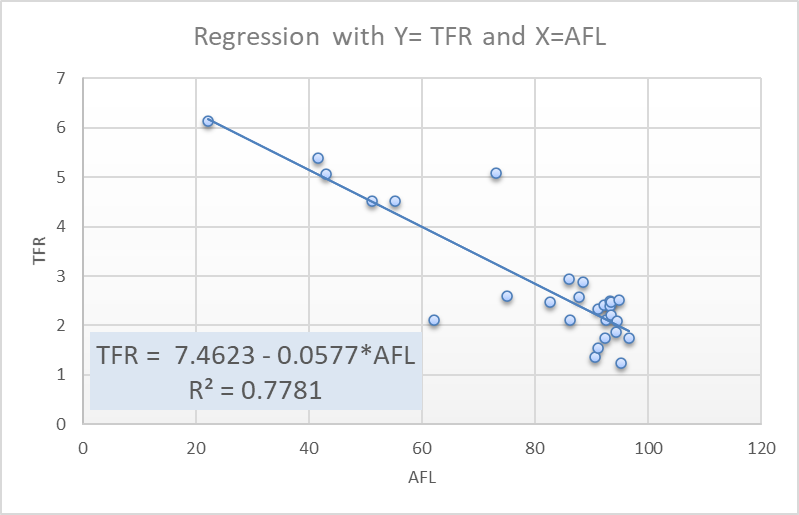
\includegraphics[scale=.75]{Reg1.png}
\end{center}
Based on the information provided on the plot, what can we tell about the correlation between the two two variables?
}}{
Ans:\MCOption[.8in]{0.882}\MCOption[.8in]{-0.882}  \MCOption[.8in]{0.7781}\MCOption[1.7in]{Can not be determined}
}{Total Score: 10}\\

\item  \QuizQuestion{ \TextInBoxOne{5.4in}{
  {\bf Statement: }  If correlation between two continuous variables is zero then the there is no relation (no linear or nonlinear relation) between the variables. 
}}{
Ans:
\MCOption{TURE} \MCOption{FALSE}

}{Total Score: 5}\\



%\item  \QuizQuestion{ \TextInBoxOne{5.4in}{
% Let us consider a simple linear regression betwen the response variable Y and the covariate X.  The fitted regression line is $\hat{Y}= 20-1.5 X$.   Let $r_{_{X,Y}}$ denotes the correlation coefficient between the variables $X$ and $Y$.  Based on the provided information idensity the correct statement among the below. 
%}}{
%Ans:$\Col{{\Row{\MCOption[1.7in]{$r_{_{X,Y}}>0$},\MCOption[1.7in]{$r_{_{X,Y}}<0$}}},{\Row{\MCOption[1.7in]{$r_{_{X,Y}}=0$},\MCOption[1.7in]{Can not be Determined}}}}$
%}{Total Score: 5}\\


\item  \QuizQuestion{ \TextInBoxOne{5.4in}{
If there is no linear relationship between two variables, then which value among the options below  would be  most appropriate about the correlation between the two variables. 
}}{
Ans:$\Row{\MCOption[1.1in]{$0.957$}, \MCOption[1.1in]{$0$},\MCOption[1.1in]{$-0.971$},\MCOption[1.1in]{$98.112$}}$
}{Total Score: 5}\\





%\item  \QuizQuestion{ \TextInBoxOne{5.4in}{
%The following table provides GDP (in Billion US\$) of Japan from 1990 to 2015 as published by The Organization for Economic Co-operation and Development (OECD):\\
%\begin{center}
%\begin{tabular}{|l|lll|}
%\hline
%               & \multicolumn{3}{l|}{Year}                                               \\ \hline
%Country   Name & \multicolumn{1}{l|}{1990}     & \multicolumn{1}{l|}{2000}    & 2010     \\ \hline
%Japan          & \multicolumn{1}{l|}{3132.818} & \multicolumn{1}{l|}{4887.52} & 5700.098 \\ \hline
%\end{tabular}
%\end{center}
%Which one among the following options most accuratly shows the Average Annual Growth Rate  (AAGR\%) of Japan between the years from 1990 to 2010?
%}}{
%Ans:\MCOption[1.1in]{$103.112\%$} \MCOption[1.1in]{$3.038\%$}\MCOption[1.1in]{$1.35\%$}\MCOption[1.1in]{$82.16\%$}
%}{Total Score: 10}\\




\item  \QuizQuestion{ \TextInBoxOne{5.4in}{
According to the World DataBank the {\bf Crude Birth Rate (CBR)} and the {\bf Crude Death Rate} for the entire world in the year 2022 is given as 16.7 (per 1000 population) and 8.9 (per 1000 population). Then what is the  world  population growth rate (in percentages) {\bf AGR}\% in the year 2021?
}}{
Ans:\MCOption[1.1in]{$78.00\%$}\MCOption[1.1in]{$7.20\%$} \MCOption[1.1in]{$0.78\%$}\MCOption[1.1in]{$0.078\%$}
}{Total Score: 5}\\

\item  \QuizQuestion{ \TextInBoxOne{5.4in}{
Consider the Lorenz curves of wealth inequality for Japan and USA.  Based on the plot below,  which country has least wealth inequality among the four?
\begin{center}
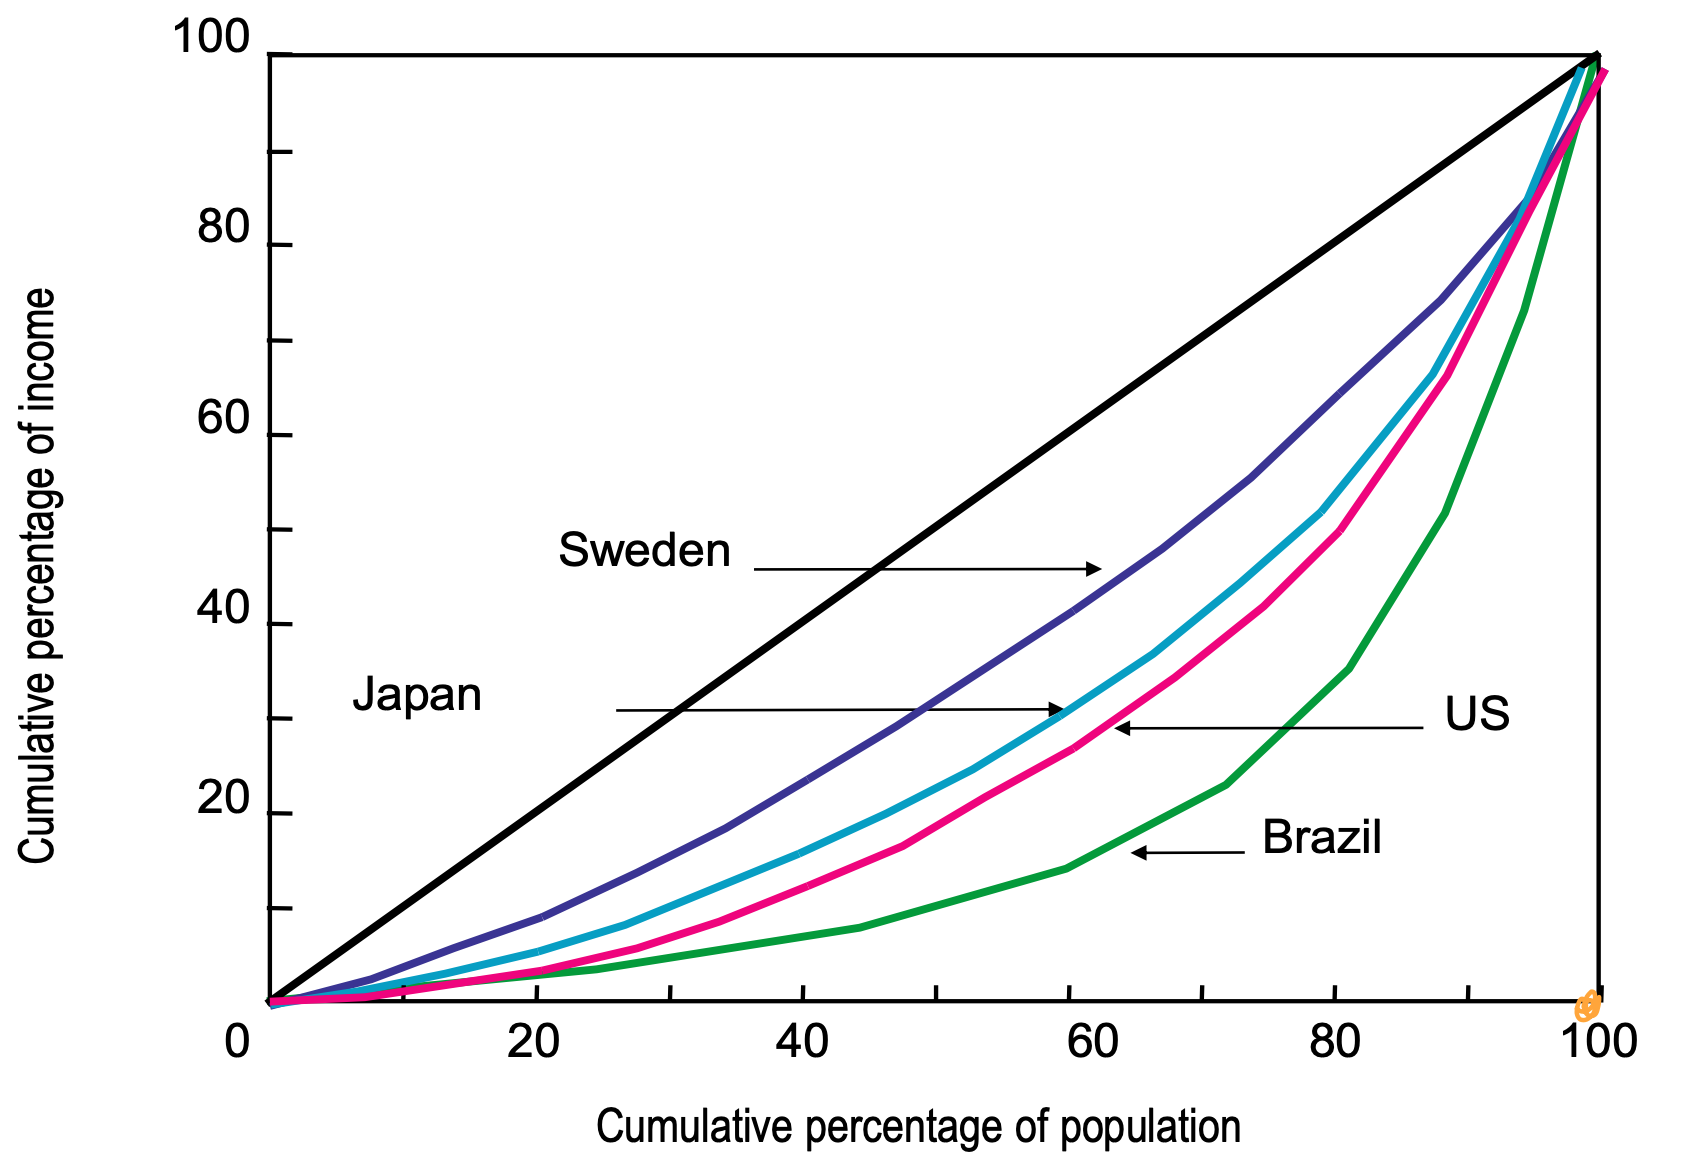
\includegraphics[scale=.29]{Lorenz.png}
\end{center}
}}{
Ans:\MCOption[1in]{Japan}\MCOption[1in]{USA}  \MCOption[1in]{Sweden}\MCOption[1in]{Brazil}
}{Total Score: 5}\\



\item  \QuizQuestion{ \TextInBoxOne{5.4in}{
Consider the histogram of `Infant Mortality Rate'  
\begin{center}
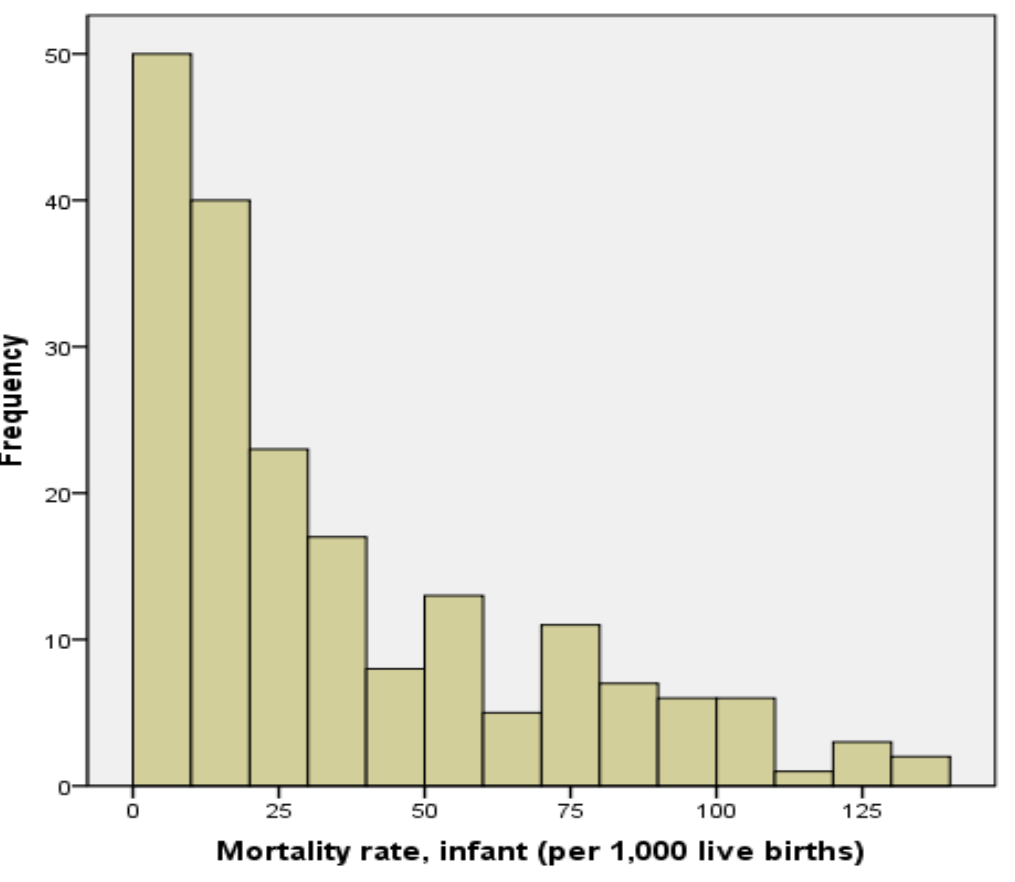
\includegraphics[scale=0.35]{Hist1.png}
\end{center}
Based on the provided histogram,  what can we say about the type of the histogram of the variable?  There may be more than one correct option.  Select all that are correct. 
}}{
Ans:
$\Col{{\Row{\MCOption[2in]{Skewed Right } , \MCOption[2in]{Skewed Left}}},{\Row{\MCOption[2in]{Mean is smaller than Median},\MCOption[2in]{Mean is larger than Median}}}}$
}{Total Score: 5}\\



\item  \QuizQuestion{ \TextInBoxOne{5.4in}{
Consider the scatter plot  of the variables `Life Expectancy at Birth' (LEB),  and `Human Development Index' (HDI) for 191 randomly selected countries.
\begin{center}
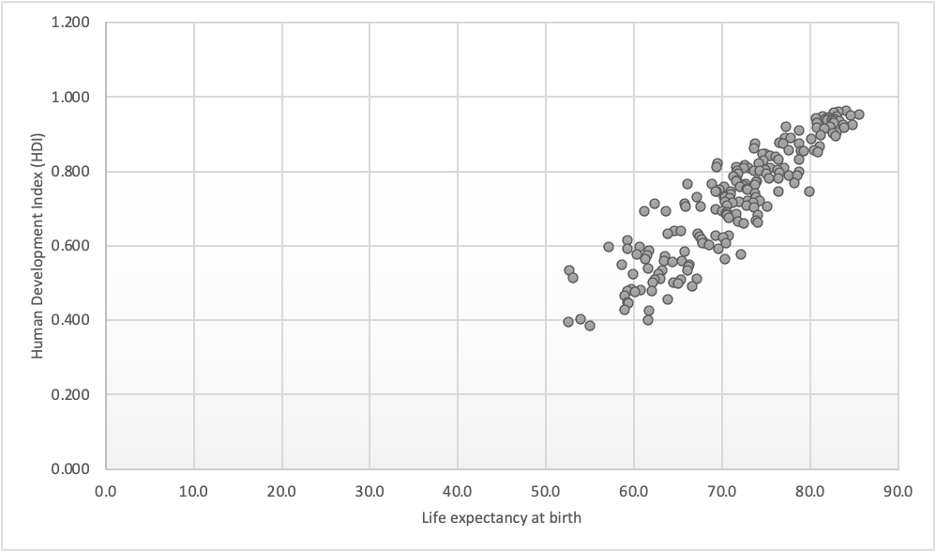
\includegraphics[scale=0.6]{ScatterHDI_LIFE.png}
\end{center}
Based on the provided scatter plot what can we say regarding the nature of association between the variables LEB, and HDI.  There may be more then one  correct statements, select all the correct options. 
}}{
Ans:
$\Col{{\Col{\MCOption[4.5in]{There is a negative linear relationship between  `LEB' and `HDI' } , \MCOption[4.5in]{There is a negative linear relationship between  `LEB' and `HDI'}}},{\Col{\MCOption[4.5in]{As `LEB'  increases, `HDI' decreases},\MCOption[4.5in]{As `LEB'  increases, `HDI' increases}, \MCOption[4.5in]{There is no relationship between  `LEB' and `HDI'. }}}}$
}{Total Score: 5}\\

\newpage


%
%
%\item \QuizQuestion{ \TextInBoxOne{5.4in}{
% {\bf Statement: }   Let $X$ and $Y$ be two random variables such that $E(X^r)= E(Y^r)$ for $r=1, 2, 3, \ldots. $Then $X$ and $Y$ are identically distributed.
%}}{
%Ans:\MCOption{TURE} \MCOption{FALSE}
%}{Total Score: 5}\\


\vspace{.1in}
\end{enumerate} 


\TextInBoxTwo[lightBlueThree]{6.5in}{ \centering  \bf\HLT[white]{ \large Part-II}\\
  \begin{center}
 Answer the following short type questions. Show your steps to get  full credit. 
 \end{center}
 %You do not need any further justification to your answers. 
 }

\item  
\begin{enumerate}
\item  \ExamQuestion{  \TextInBoxOne{5.75in}{ 
The population of UAE was 6.988 million in 2008 and 9.441 million in 2022.  The calculated AAGR\% during the period is $1.0217$.  {\bf Calculate the {\it \bf Doubling Time (DT)} of the UAE population if the AARG\% remains same. }
}}{\vspace{.1in}
}{\hspace{-.2in}Total Score: 5}\\
\vspace{1.2in}

\item  \ExamQuestion{  \TextInBoxOne{5.75in}{The Adult Female Literacy Rate (\%) for a seven selected under developed countries are provided as below: 
$$\Row{43.1{,},	51.2{,},	55.2{,},	62.3{,},	73.1{,},	75.0{,},	82.8}$$
{\bf What is the median of the above seven numbers?}
}}{\vspace{.1in}
}{\hspace{-.2in}Total Score: 5}\\
\vspace{1in}


\item  \ExamQuestion{  \TextInBoxOne{5.75in}{Calculate Weighted Average
}}{\vspace{.1in}
}{\hspace{-.2in}Total Score: 5}\\
\vspace{2in}


\item  \ExamQuestion{  \TextInBoxOne{5.75in}{Frequency Distribution Table To histogram
}}{\vspace{.1in}
}{\hspace{-.2in}Total Score: 5}\\
\vspace{2in}

%
%\item  \ExamQuestion{  \TextInBoxOne{5.75in}{WRLI
%}}{\vspace{.1in}
%}{\hspace{-.2in}Total Score: 5}\\
%\vspace{2in}


\end{enumerate}




\newpage



\item[4.]  \TextInBoxTwo[lightBlueTwo]{6.25in}{ 
 Consider the following table on  world total population provided on a few years interval from 1980 to 2015\\
 \TextInBoxOne{6in}{
 \begin{center}
\begin{tabular}{|l|c|}
\hline
 Year & World Population  \\
  &  {\tiny(in billions)} \\ \hline\hline
1980                                  & 4.44    \\ \hline
1990                                 & 5.29   \\ \hline
2000                                  & 6.12 \\ \hline
2015                                  & 7.34     \\ \hline
\end{tabular}
\end{center}
 }
}
\begin{enumerate}
\item \ExamQuestion{ \TextInBoxOne{5.7in}{	Find the  Average Annual Growth Rate  {\bf (AAGR\%)} for  world population during the period {\bf from  1980 to the year 2015. }
}}{ \\
}{\hspace{-.2in}Total Score: 10 }\\
\vspace{2in}
\item \ExamQuestion{ \TextInBoxOne{5.7in}{ {\bf Predict the globalpopulation  in the year {\bf 2035} using  2015 as the base year. } Assume that the AAGR\% for world population  remains fixed at the value  that you have calculated in part (a) of this problem. 
}}{ \\
}{\hspace{-.2in}Total Score: 10}\\
\vspace{2in}\\

\end{enumerate}




\newpage

\item[4.]  \TextInBoxTwo[lightBlueTwo]{6.25in}{ To Estimate the average life expectancy in {\bf less-Developed countries}, a random sample of 144 less developed countries reveals the following data.
$\text{Sample size:} 144, \text{Mean:}  67.1 \text{Standard deviation:} 28.9$\\
On the other hand,  the average life expectancy in Developed countries, a random sample of 144 {\bf developed countries} reveals the following data.
$\text{Sample size:} 144, \text{Mean:}  76 \text{Standard deviation:}28.9$\\
}
\begin{enumerate}
\item \ExamQuestion{ \TextInBoxOne{5.7in}{	Compute the 95\% confidence interval for the average life expectancy in less-developed countries.
}}{ \\
}{\hspace{-.2in}Total Score: 10 }\\
\vspace{2in}
\item \ExamQuestion{ \TextInBoxOne{5.7in}{Compute the 95\% confidence interval for the average life expectancy in developed countries.
}}{ \\
}{\hspace{-.2in}Total Score: 10}\\
\vspace{2in}\\
\item \ExamQuestion{ \TextInBoxOne{5.7in}{Explain whether there is a difference in the life expectancy between less developed and developed countries.
}}{ \\
}{\hspace{-.2in}Total Score: 10}\\
\vspace{2in}\\

\end{enumerate}

\newpage








\item[5.] \TextInBoxTwo[lightBlueTwo]{6.25in}{ 
 \TextInBoxOne{6.1in}{The following table is a hypothetical population of 100 individuals with a maximum life span of 4 years, using the remaining life expectancy method:\\
\begin{center}
\begin{tabular}{|l|l|l|}
\hline
\hline
x & $l_x\hspace{.4in}$ & $  d_x  \hspace{.4in}$  \\ \hline\hline
0 & 100  & 25        \\ \hline
1 &      & 10         \\ \hline
2 &      & 25        \\ \hline
3 &      & 40       \\ \hline
4 &      & 0          \\ \hline
\end{tabular}\\
\vspace{.1in}
\end{center} 
}}

\begin{enumerate}
\item \ExamQuestion{ \TextInBoxOne{5.7in}{Complete the following table corresponding o the Remaining Life Expectancy.\\
}}{% \begin{center}
\vspace{.2in}
\\
{\Huge 
\begin{tabular}{|l|l|l|l|l|l|}
\hline
x & $l_x\hspace{.75in}$ & $  d_x  \hspace{.75in}$ & $     L_x\hspace{.75in} $ & $   T_x   \hspace{.75in} $ & $    e_x \hspace{.75in}  $ \\ \hline
0 & 100  & 25   &      &      &      \\ \hline
1 &      & 10   &      &      &      \\ \hline
2 &      & 25   &      &      &      \\ \hline
3 &      & 40   &      &      &      \\ \hline
4 &      & 0    &      &      &      \\ \hline
\end{tabular}
}
\vspace{1in}
%\end{center}
}{\hspace{-.2in}Total Score: 10}\\
\item \ExamQuestion{ \TextInBoxOne{5.7in}{What is the life expectancy at birth of this hypothetical population?
}}{ \\
}{\hspace{-.2in}Total Score: 5 }\\




\end{enumerate}



\newpage


\item[5.] \TextInBoxTwo[lightBlueTwo]{6.25in}{ 
 \TextInBoxOne{6.1in}{
Consider an example of the income distribution given by. \\
\begin{tabular}{|l|l|}
\hline
                                  & Income \%  \\ \hline
Income share held by lowest 20\%  & 10       \\ \hline
Income share held by second 20\%  & 15                              \\ \hline
Income share held by third 20\%   & 20                              \\ \hline
Income share held by fourth 20\%  & 25        \\ \hline
Income share held by highest 20\% & 30         \\ \hline
\end{tabular}
}}
\begin{enumerate}
\item \ExamQuestion{ \TextInBoxOne{5.7in}{Compute the table with the cumulative percentages of Income Share ans the corresponding cumulative percentages of population and complete the Table Below 
}}{ \\ \Large
\begin{tabular}{|l|l|}
\hline
                              Cumulative Population \% & Cumulative \% Income \\ \hline
  \hspace{1in}&  \hspace{1in}                           \\ \hline
     &                      \\ \hline
        &                      \\ \hline
       &                      \\ \hline
      &                      \\ \hline
\end{tabular}
}{\hspace{-.2in}Total Score: 10}\\

\item \ExamQuestion{ \TextInBoxOne{5.7in}{Plot the Lorenz curve of this hypothetical country.
}}{ \\
}{\hspace{-.2in}Total Score: 5 }\\


\newpage

\item \ExamQuestion{ \TextInBoxOne{5.7in}{Compute the Gini's Index using the table provided above.
}}{ \\\Large
\begin{tabular}{|l|l|l|l|l|l|}
\hline
Decile & $f_i$\hspace{.7in} & $x_i$\hspace{.7in} & $y_i\hspace{.7in}$ & $(y_i+y_{i-1})$ & $f_i\times (y_i+y_{i-1})$ \\ \hline \hline
20     &   20   & 10     &      &               &                   \\ \hline
40     &      20&  15    &      &               &                   \\ \hline
60     &      20&   20   &      &               &                   \\ \hline
80     &      20&    25  &      &               &                   \\ \hline
100    &      20&    30  &      &          &                   \\ \hline
    &      &      &      & Total         &                   \\ \hline
\end{tabular}
}{\hspace{-.2in}Total Score: 5 }\\
Here $y_i$ denotes the cumulative income share that you have computed in the previous part of the problem. 

${\Huge G}=$

\end{enumerate}



\newpage

\item[5.] \TextInBoxTwo[lightBlueTwo]{6.25in}{ 
 \TextInBoxOne{6.1in}{Consider a data set containing two continuous variables,  `Mean years of schooling' and `Human Development Index' (HDI)  of a sample of 192 countries.  For a regression model `Human Development Index' is considered to be the response variable (Y) while the corresponding   `Mean years of schooling' (X) is used as a covariate/independent variable.  The following is the scatter plot of the two variables. 
 \begin{center}
 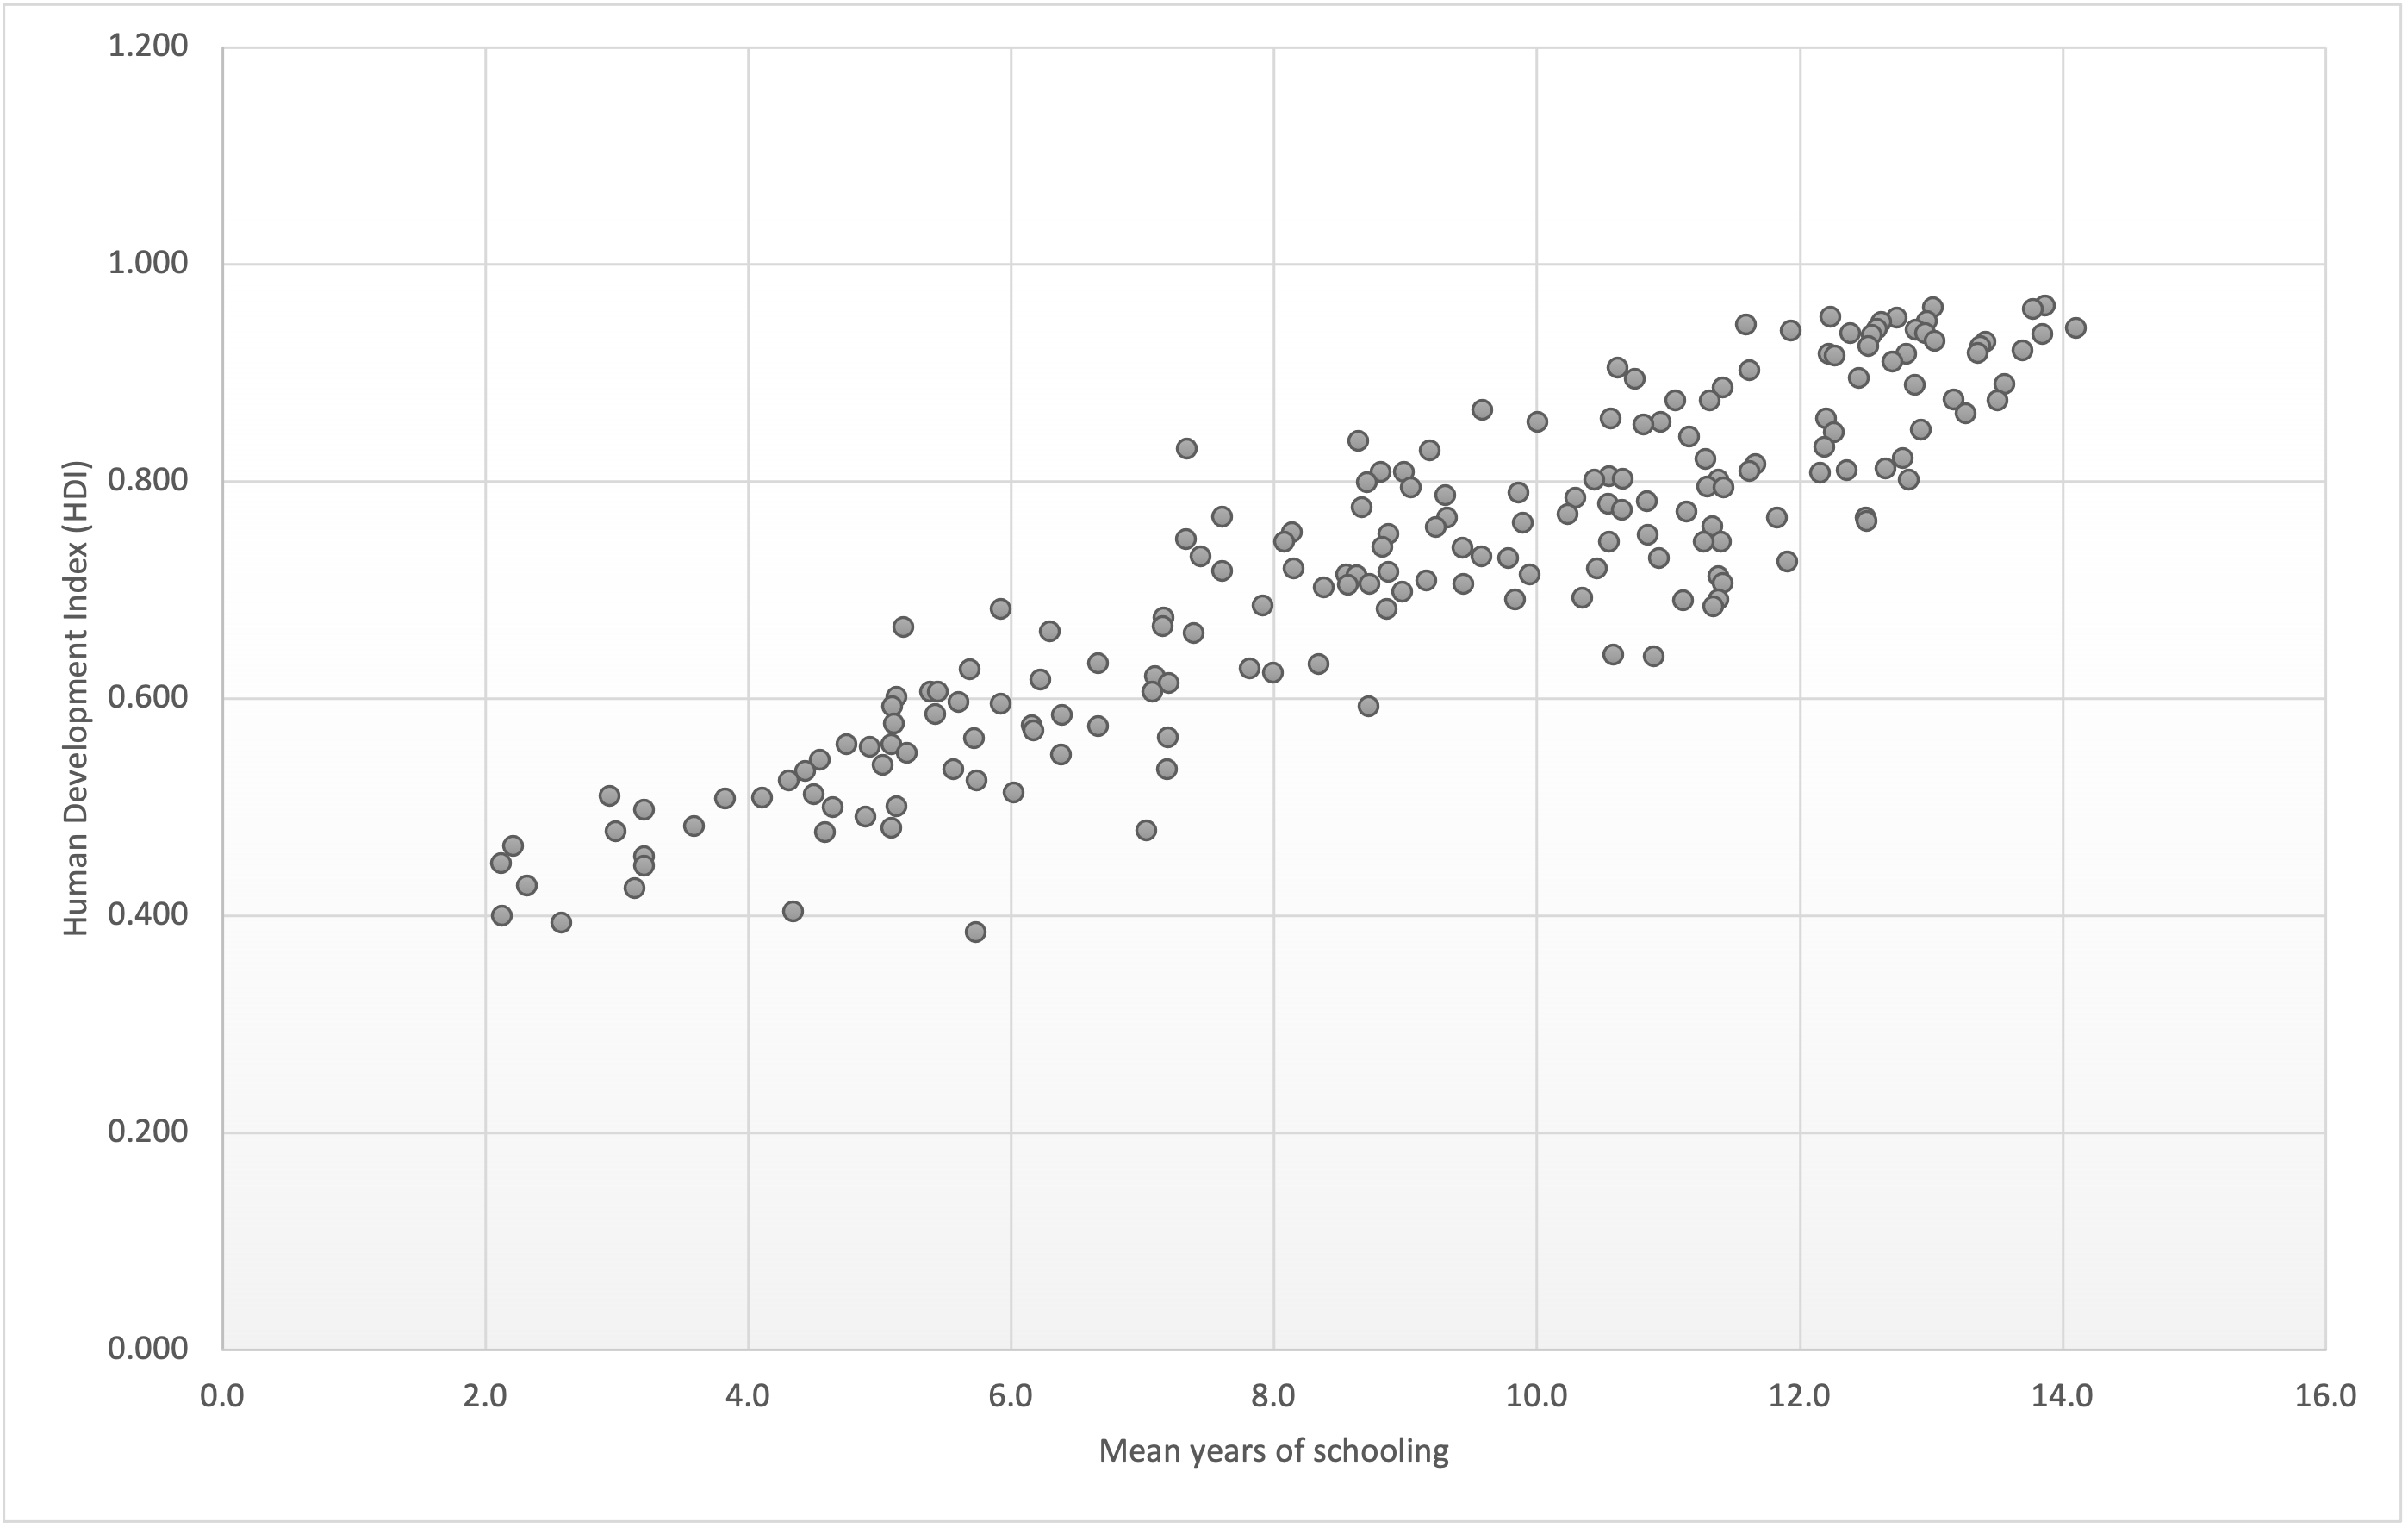
\includegraphics[scale=.5]{LineSchoolHDI.png}
 \end{center}
 Based on the data, the following summary of the variables are obtained:\\
%\begin{center}
%\begin{tabular}{|l|l|l|l|l|}
%\hline
%$\bar{X}$       & $\bar{Y}$        & $S_X$     & $S_Y$     & $r_{_{XY}}$    \\ \hline
%8.99  & 0.72 & 3.17 & 0.15 & 0.9091\\ \hline
%\end{tabular}
%\end{center}
\begin{center}
\begin{tabular}{|c|c|c|}
\hline
      & \multicolumn{1}{c|}{\textbf{Mean years of   schooling}} & \multicolumn{1}{c|}{\textbf{Human   Development Index (HDI)}} \\ \hline\hline
Sample Mean  & $\bar{X}=8.99$                                                    &$ \bar{Y}=0.72  $                                                        \\ \hline
Sample Standard Deviation & $S_X=3.17$                                                    & $S_Y=0.15$                                                          \\ \hline
\end{tabular}\\
\vspace{.1in}
\begin{tabular}{|l|l|}
\hline
Correlation between the variables  & $r_{_{XY}}=0.9091$ \\ \hline
\end{tabular}
\end{center}
Finally we consider a simple  linear regression model: $\hat{Y}= a+bX$ where $a$ and $b$ denotes the intercept and the slope correspondingly. 
Based on the information provided,  answer the following questions: 
}}

\begin{enumerate}
%\item \ExamQuestion{ \TextInBoxOne{5.7in}{Compute the correlation between the variables `Average Life Expectancy' and `Adult Female Literacy rate'.
%}}{ \\ 
%}{\hspace{-.2in}Total Score: 10}\\

\item \ExamQuestion{ \TextInBoxOne{5.7in}{Compute the value of the {\bf slope} and provide its {\bf interpretation}. 
}}{ 
}{\hspace{-.2in}Total Score: 5 }\\

\item \ExamQuestion{ \TextInBoxOne{5.7in}{Compute the value of the intercept and provide its interpretation.  Is the interpretation meaningful in the  context of the current example?
}}{ 
}{\hspace{-.2in}Total Score: 5 }\\


\item \ExamQuestion{ \TextInBoxOne{5.7in}{Based on the computed regression equation, predict the `Human   Development Index'  of a country for which the corresponding `Mean years of   schooling' is 10.
}}{ 
}{\hspace{-.2in}Total Score: 5 }\\



\end{enumerate}









%
%
%\item  \TextInBoxOne{6in}{ 
% An oil exploration firm is formed with enough capital to finance ten explorations. The probability
%of a particular exploration being successful is 0.1. Assume the explorations are independent.
%}
%\begin{enumerate}
%\item \ExamQuestion{ \TextInBoxOne{5.4in}{
%Find the mean and variance of the number of successful explorations.
%}}{ \\
%}{\hspace{-.2in}Total Score: 5 }\\
%\vspace{4in}
%
% \ExamQuestion{ \TextInBoxOne{5.4in}{ \item 
%Suppose the firm has a fixed cost of \$20,000 in preparing equipment prior
%to doing its first exploration. If each successful exploration costs \$30,000 and each unsuccessful
%exploration costs \$15,000, find the expected total cost to the firm for its ten explorations.
%}}{ \\
%}{\hspace{-.2in}Total Score: 5 }\\
%\vspace{4in}
%\end{enumerate}

 \newpage
%\ExamQuestion{    \item \TextInBoxOne{5.7in}{
%In responding to a survey question on a sensitive topic (such as “ Have you ever tried
%cigarette?”), many people prefer not to respond in the affirmative. Suppose that 80\% of
%the population have not tried cigarette and all of those individuals will truthfully answer no
%to your question. The remaining 20\% of the population have tried cigarette and 70\% of those
%individuals will lie. Derive the probability distribution of Y , the number of people you would
%need to question in order to obtain a single affirmative response. 
%  }}{ \\ 
%}{\hspace{-.2in}Total Score: 5}\\


%
%\item[6.]  \ExamQuestion{  \TextInBoxOne{5.75in}{ Consider the following table that provides the Unit Price and Production Quantities of Item-A, B and C  in the years 2006, and 2016. 
%\begin{center}
%\begin{tabular}{|l|ll|ll|}
%\hline
%     & \multicolumn{2}{l|}{Unit Price}  & \multicolumn{2}{l|}{Output quantities}                              \\ \hline
%Item/Year & \multicolumn{1}{l|}{ 2006} & 2016 & \multicolumn{1}{l|}{2006} & 2016 \\ \hline
%Item-A    & \multicolumn{1}{l|}{45}                           & 50   & \multicolumn{1}{l|}{400}                          & 700                          \\ \hline
%Item-B    & \multicolumn{1}{l|}{30}                           & 38   & \multicolumn{1}{l|}{216}                          & 350                          \\ \hline
%Item-C    & \multicolumn{1}{l|}{40}                           & 45   & \multicolumn{1}{l|}{300}                          & 800                          \\ \hline
%\end{tabular}\\
%\end{center}
%{\bf Question: } Calculate the Laspeyres Price Index,  show all the steps. 
%}}{ \\\vspace{.1in}
%}{\hspace{-.2in}Total Score: 15}\\
%\vspace{2in}


\end{enumerate}



%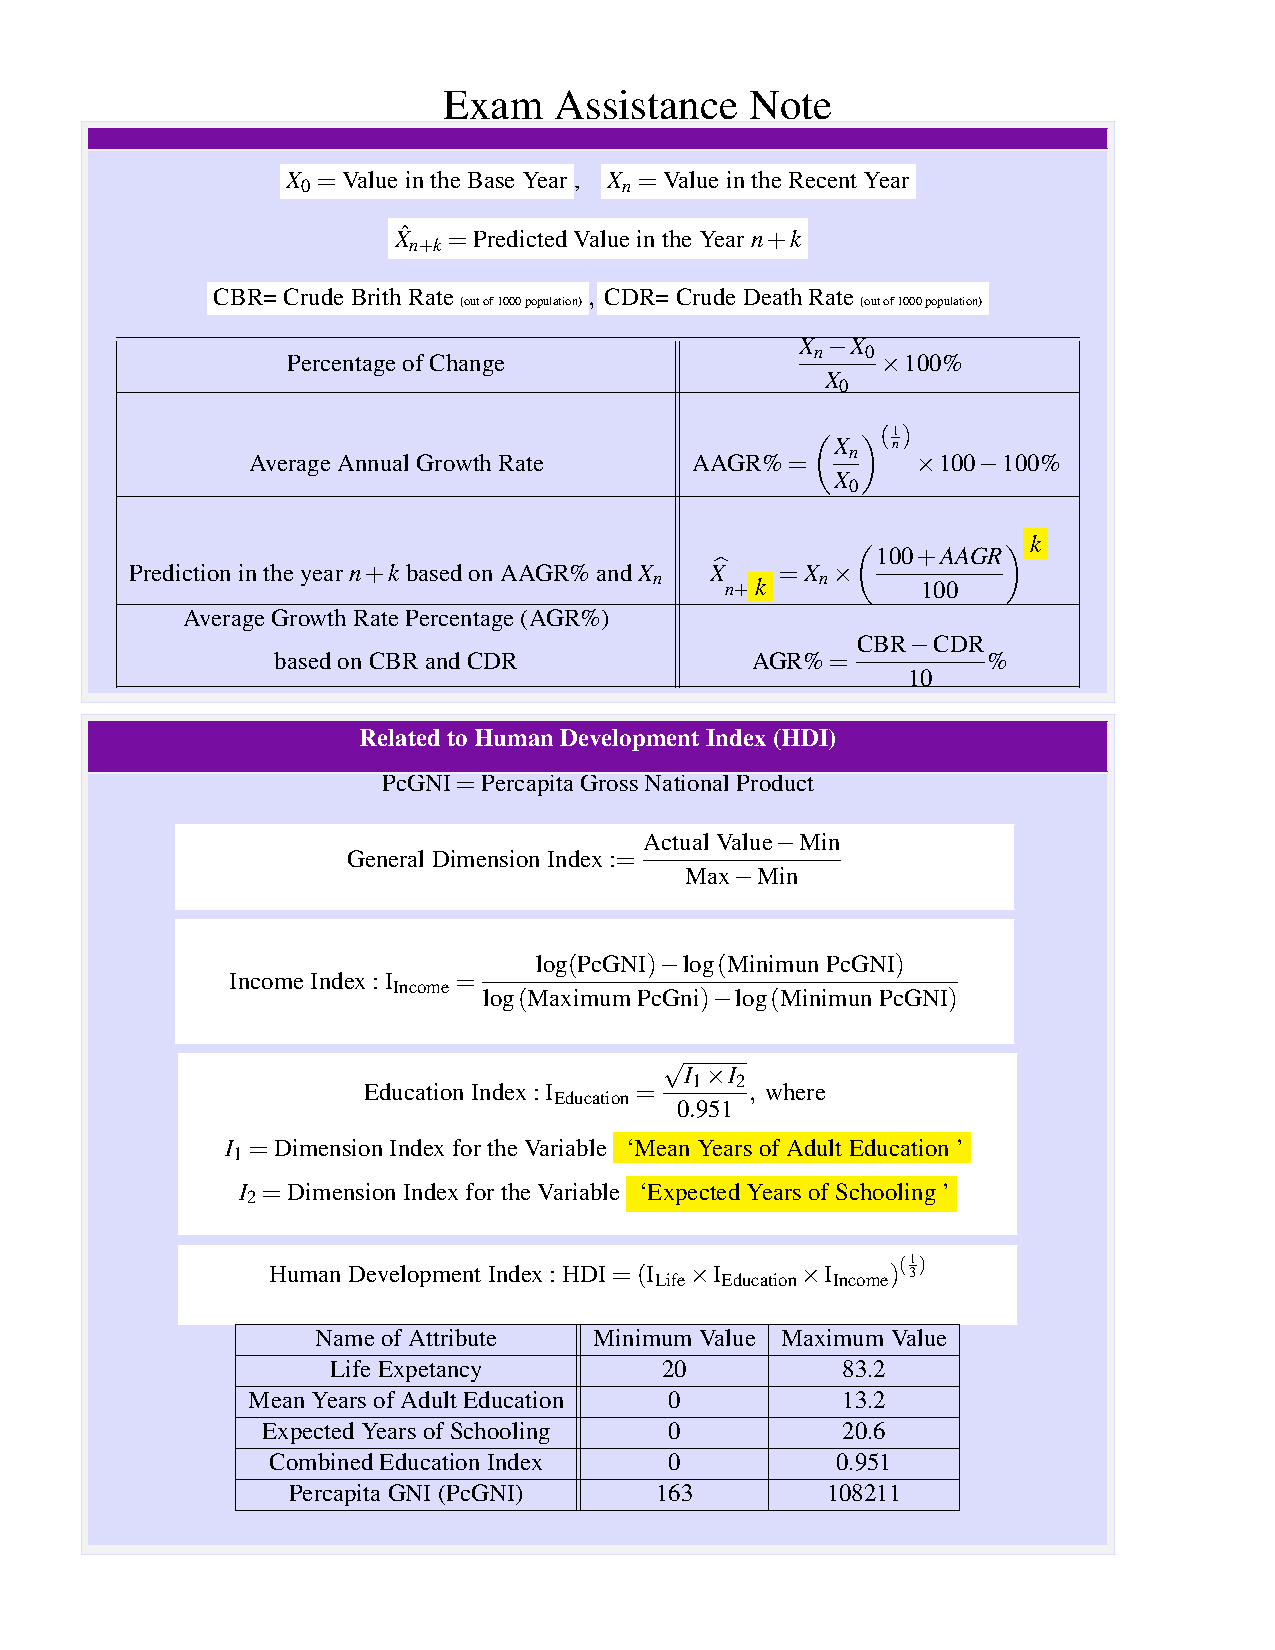
\includepdf[pages=-]{ExamAssistanceNote_STAt101.pdf}






\end{document}